
\chapter{维数}
\label{ch:dimension}

\epigraph{人人都知道什么是曲线——直到他学了足够多的数学、陷入困惑为止。}{——F.~\trKlein，[RS, p.~90]}

到这一步，你对\trScheme{}已经知道得不少，但有些根本性的观念你还无法定义。特别地，「光滑\trSurface」这个短语你还用不了，因为它牵涉\trDimension{}与\trSmoothness{}两个观念。我们走了这么远竟然都没用上这些想法，你也许会感到惊讶。这些观念居然还挺微妙，你也可能会为之不安；但请记住：在数学的所有分支里，它们都是微妙的。

本章将处理第一个观念，即\trScheme{}的\trDimension。它应当与我们的几何直觉相吻合，并把后者推广。尽管我们把\trDimension{}当作几何学中的基本观念，它却是个滑溜溜的概念——一如它在整个数学中的样子。即使在线性代数里，\trVectorSpace{}之\trDimension{}的定义初见之下也令人吃惊，尽管它很快就会变成第二天性。\trManifold{}的\trDimension{}定义同样不那么平凡。例如，我们凭什么知道某个二维\trManifold{}与某个三维\trManifold{}之间不存在\trIsomorphism？你的回答多半要用到\trTopology，所以\trDimension{}的观念往往颇有\trTopology{}味道，这一点不该让你意外。

给在复数上思考的读者一句提醒：我们的\trDimension{}将是代数的，因而是「实」图景的一半。例如，我们很快就会看到：$\mathbb{A}^1_{\mathbb{C}}$——你可以把它想成复数（外加一个\trGenericPoint）——的\trDimension{}是 $1$。


\section{维数与余维}

\textbf{12.1.1.}\ \emph{\trhDefinition{}（们）：\trDimension{}。}\quad 出人意料的是，正确的定义竟是纯拓扑的——它只依赖于\trTopologicalSpace{}本身，而不依赖于\trStructureSheaf。我们把\trTopologicalSpace{} $X$ 的\textbf{\trDimension}（记作 $\dim X$）定义为诸\trIrreducible{}\trClosedSet{}之链的长度的上确界，其中诸不可约闭集自 $0$ 起编号。（\trDimension{}可以是无穷的。）研究空集的学者不妨把空集的\trDimension{}取作 $-\infty$。（一个来自线性代数的类比：\trVectorSpace{}的\trDimension{}是诸子空间之链的长度的上确界。）把一个\trRing{}的\trDimension{}定义为诸嵌套\trPrimeIdeal{}之链的长度的上确界（编号自零起）。\trDimension{}的这两版定义有时被称为\textbf{\trKrullDimension}（Krull dimension）。（你也许会认为\trNoetherian{}环必具有有限的\trDimension{}，因为\trPrimeIdeal{}的链都是有限的——但这并不必然成立，见\mbox{练习~12.1.M}。）

\textbf{12.1.A.（容易的练习）}\quad 证明：$\dim\Spec A=\dim A$。（提示：\cref{ex:irreducible-prime-bijection}给出了 $\Spec A$ 的诸\trIrreducible{}\trClosedSubset{}与 $A$ 的诸\trPrimeIdeal{}之间的一个双射。这个双射是「反转包含关系」的。）

$\Spec A$ 与 $\Spec A/\mathfrak{N}(A)$ 之间的\trHomeomorphism{}（\S3.4.7：\trZariskiTopology{}不理会\trNilpotent{}元）蕴涵 $\dim\Spec A=\dim\Spec A/\mathfrak{N}(A)$。

\textbf{12.1.2.}\ \emph{\trhExample{}。}\quad 我们已经辨认出 $k[t]$ 的全部\trPrimeIdeal{}（它们是 $0$，以及对\trIrreducible{}多项式 $f(t)$ 的 $(f(t))$）、$\mathbb{Z}$ 的全部\trPrimeIdeal{}（$(0)$ 与诸 $(p)$）、$k$ 的全部\trPrimeIdeal{}（只有 $(0)$），以及 $k[x]/(x^2)$ 的全部\trPrimeIdeal{}（只有 $(x)$），于是可以迅速核验：$\dim\mathbb{A}^1_k=\dim\Spec\mathbb{Z}=1$，$\dim\Spec k=0$，$\dim\Spec k[x]/(x^2)=0$。

\textbf{12.1.3.}\quad 对可约空间而言，\trDimension{}这个观念必须小心对待。若 $Z$ 是两个\trClosedSubset{} $X$ 与 $Y$ 的并，则 $\dim Z=\max(\dim X,\dim Y)$。从而\trDimension{}并不是一个空间的「局部」特征。这件事有时令我们困扰，所以我们尽量只谈\trIrreducible{}\trTopologicalSpace{}的\trDimension。我们说一个\trTopologicalSpace{}是\textbf{\trPureDimensional{}的}（pure dimensional）或\textbf{\trEquidimensional{}的}（equidimensional）（相应地，具有\textbf{\trPureDimension{} $n$}（pure dimension $n$）或\textbf{维数为 $n$ 的\trEquidimensional}（equidimensional of dimension $n$）），若它的每个\trIrreducibleComponent{}都具有相同的\trDimension（相应地，它们全都具有\trDimension{} $n$）。\trPureDimension{} $1$（相应地，$2$、$n$）的\trTopologicalSpace{}称为一条\textbf{\trCurve}（相应地，一张\textbf{\trSurface}、一个\textbf{\trNFold}（$n$-fold））。

\textbf{12.1.B.（有用的练习）}\quad 证明：一个\trScheme{}的\trDimension{}为 $n$，当且仅当它有一个由\trDimension{}至多为 $n$ 的\trAffine\trOpenSubset{}构成的\trOpenCover，并且等号在其中某个\trAffine\trOpenSubset{}上达到。提示：你或许会发现，证明下面这件事在此处和日后都有帮助。对任意\trTopologicalSpace{} $X$ 与\trOpenSubset{} $U\subset X$，$U$ 的诸\trIrreducible{}\trClosedSubset{}与 $X$ 的同 $U$ 相交的诸\trIrreducible{}\trClosedSubset{}之间存在一个双射。

\textbf{12.1.C.（容易的练习）}\quad 证明：\trDimension{}为 $0$ 的\trNoetherian\trScheme{}只有有限多个点。

\textbf{12.1.D.（容易的练习）}\quad 证明：具有同一有限\trDimension{}的诸\trIntegralDomain{}之间的\trSurjectiveMap{}必是\trIsomorphism。

\textbf{12.1.E.（练习：\trIntegral{}态射的纤维；\S8.3.8 中所许诺的）}\quad 设 $\pi\colon X\to Y$ 是一个\trIntegral{}态射。证明：$\pi$ 的每个（非空）\trFiber{}的\trDimension{}都是 $0$。提示：由于\trIntegral{}态射对\trBaseChange{}保持（\mbox{练习~10.4.D(d)}），我们可以假设 $Y=\Spec k$。于是要证的就是：若 $\phi\colon k\to A$ 是一个\trIntegralExtension，则 $\dim A=0$。证明概要：设 $\mathfrak{p}\subset\mathfrak{m}$ 是 $A$ 的两个\trPrimeIdeal。对 $\mathfrak{p}$ 取商，便可假设 $A$ 是\trIntegralDomain。我断言：任何非零元素都是\trInvertible{}的。比如说 $x\in A$ 且 $x\neq0$。那么 $x$ 的\trMinimalPolynomial（首一的）具有非零常数项。但这样一来 $x$ 就\trInvertible{}了——回想这些系数位于一个\trField{}之中。

\textbf{12.1.F.（重要练习）}\quad 证明：若 $\pi\colon\Spec A\to\Spec B$ 相应于诸\trRing{}的一个\trIntegralExtension，则 $\dim\Spec A=\dim\Spec B$。提示：证明「楼下」的一条\trPrimeIdeal{}链借 Going-Up 定理（\cref{ex:going-up-theorem}）给出「楼上」的一条等长的链。反过来，「楼上」的一条链给出「楼下」的一条链。用\mbox{练习~12.1.E}证明：「楼上」这条链的任何两个元素都不会被送到「楼下」这条链的同一个元素 $[\mathfrak{q}]\in\Spec B$ 上。

\textbf{12.1.G.（练习）}\quad 证明：若 $\nu\colon\widetilde{X}\to X$ 是一个\trScheme{}的\trNormalization（可能是在 $X$ 的\trFunctionField{}的某个\trFiniteFieldExtension{}中取的），则 $\dim\widetilde{X}=\dim X$。为方便起见，你尽管假设 $X$ 是\trIntegral{}的。

\textbf{12.1.H.（有用的练习）}\quad 设 $X$ 是一个仿射 $k$-\trScheme，而 $K/k$ 是一个\trAlgebraic\trFieldExtension。
\begin{enumerate}[label=(\alph*)]
\item 设 $X$ 具有\trPureDimension{} $n$。证明：$X_K:=X\times_k K$ 具有\trPureDimension{} $n$。（一个推广见\mbox{练习~24.5.F}，它比方说去掉了仿射假设。向任意\trFieldExtension{}的种种可能推广的命运如何，另见\mbox{练习~12.2.M}与注记~12.2.17。）提示：若 $X=\Spec A$，化归到 $A$ 是\trIntegralDomain{}的情形。$X_K$ 的一个\trIrreducibleComponent{}对应于 $A_K:=A\otimes_k K$ 的一个\trMinimalPrime{} $\mathfrak{p}$。设 $a\in\ker(A\to A_K/\mathfrak{p})$。利用下面两件事证明 $a=0$：$a$ 落在 $A_K$ 的一个\trMinimalPrime{} $\mathfrak{p}$ 中（从而由 \S6.6.23 它是\trZerodivisor），并且 $A_K$ 是一个自由 $A$-\trModule（于是只要 $a\in A$ 非零，在 $A_K$ 中用 $a$ 相乘就是单的）。这样便知 $A\to A_K/\mathfrak{p}$ 是单的。随后用\mbox{练习~12.1.F}。
\item 证明 (a) 的逆命题：证明：若 $X_K$ 具有\trPureDimension{} $n$，则 $X$ 具有\trPureDimension{} $n$。
\end{enumerate}

\textbf{12.1.I.（练习）}\quad 证明：$\dim\mathbb{Z}[x]=2$。（提示：$\mathbb{Z}[x]$ 的诸\trPrimeIdeal{}曾在\cref{ex:affine-space-over-z-picture}中被隐含地确定过。）

\textbf{12.1.4.\ \trCodimension。}\quad 由于\trDimension{}在\trDisjointUnion{}之下表现古怪，我们在定义\trCodimension{}以及使用这个词时都需要一些小心。例如，若 $Y$ 是 $X$ 的一个\trClosedSubset，我们或许会把\trCodimension{}定义为 $\dim X-\dim Y$，但这种定义表现很糟。比如说，若 $X$ 是一个点 $Y$ 与一条\trCurve{} $Z$ 的\trDisjointUnion，则 $\dim X-\dim Y=1$，但这同 $X$ 在 $Y$ 附近的局部行为毫无关系。

更好的定义如下。为了避免过多的病理，我们\emph{只}在 $Y$ \trIrreducible{}时才定义 $Y$ 在 $X$ 中的\trCodimension。（在任何别的场合使用这个词时，务必要极端小心。）\trTopologicalSpace{}的\trIrreducible{}子集 $Y\subset X$ 的\textbf{\trCodimension}{}定义为：以 $\overline{Y}$ 打头的\trIrreducible{}\trClosedSubset{}\emph{递增}链之长度的上确界（编号自 $0$ 起——回想：\trIrreducible{}集合的\trClosure{}仍是\trIrreducible{}的，\cref{ex:irreducible-open-dense}(b)）。特别地，一个点的\textbf{\trCodimension}{}就是它的\trClosure{}的\trCodimension。$Y$ 在 $X$ 中的\trCodimension{}记作 $\operatorname{codim}_X Y$。

我们说，\trRing{}中\trPrimeIdeal{} $\mathfrak{p}$ 的\textbf{\trCodimension}{}等于自 $\mathfrak{p}$ 出发的递降\trPrimeIdeal{}链之长度的上确界，编号自 $0$ 起。于是在\trIntegralDomain{}中，理想 $(0)$ 的\trCodimension{}为 $0$；而在 $\mathbb{Z}$ 中，理想 $(23)$ 的\trCodimension{}为 $1$。注意：$A$ 中\trPrimeIdeal{} $\mathfrak{p}$ 的\trCodimension{}是 $\dim A_{\mathfrak{p}}$（见 \S3.2.9）。（这个观念常被称为\textbf{\trHeight}。）从而，$\mathfrak{p}$ 在 $A$ 中的\trCodimension{}就是 $[\mathfrak{p}]$ 在 $\Spec A$ 中的\trCodimension。

（继续与线性代数的类比：向量子空间 $Y\subset X$ 的\trCodimension{}是以 $Y$ 打头的子空间递增链之长度的上确界。这个定义比 $\dim X-\dim Y$ 好，因为即便当 $\dim X=\infty$ 时它也管用。你或许更愿意把 $\operatorname{codim}_X Y$ 定义为 $\dim(X/Y)$；那就好比把 $\mathfrak{p}$ 在 $A$ 中的\trCodimension{}定义为 $A_{\mathfrak{p}}$ 的\trDimension{}——见上一段。）

\textbf{12.1.J.（练习）}\quad 证明：若 $Y$ 是\trScheme{} $X$ 的一个\trIrreducible{}\trClosedSubset，而 $\eta$ 是 $Y$ 的\trGenericPoint，则 $Y$ 的\trCodimension{}就是\trLocalRing{} $\OO_{X,\eta}$ 的\trDimension。

\textbf{12.1.5.}\quad 注意：若 $Y$ 是 $X$ 的一个\trIrreducibleComponent，则 $Y$ 在 $X$ 中的\trCodimension{}为 $0$。类似地，若 $Y$ 不是\trIrreducibleComponent，并且对它所含于的每个\trIrreducibleComponent{} $Y'$，在 $Y$ 与 $Y'$ 之间都不存在严格介于其间的\trIrreducible{}\trClosedSubset，则 $Y$ 的\trCodimension{}为 $1$。（例子见\cref{fig:codim-behavior}。）一个\trClosedSubset，若它的全部\trIrreducibleComponent{}在某个环绕空间 $X$ 中的\trCodimension{}都是 $1$，就称为 $X$ 中的\textbf{\trHypersurface}。（小心：「\trHypersurface」一词在代数几何中可以指略有不同的东西，而且各有全然合理的缘由；例如见定义~9.3.2。）

\begin{figure}[htbp]
\centering
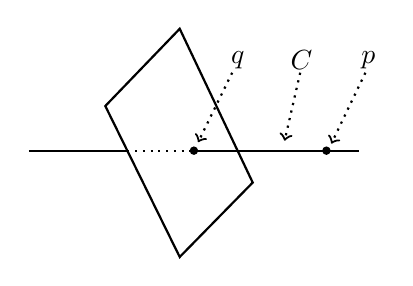
\begin{tikzpicture}[scale=0.9,line width=0.8pt]
  \draw (-0.2,1.72) -- (0.83,-0.45) -- (-0.2,-1.5) -- (-1.25,0.63) -- cycle;
  \draw (-2.33,0) -- (-0.94,0);
  \draw[dotted] (-0.94,0) -- (0,0);
  \draw (0,0) -- (2.33,0);
  \fill (0,0) circle (1.7pt);
  \fill (1.87,0) circle (1.7pt);
  \node at (0.62,1.28) {$q$};
  \draw[dotted,->] (0.54,1.1) -- (0.06,0.12);
  \node at (1.52,1.28) {$C$};
  \draw[dotted,->] (1.5,1.1) -- (1.28,0.14);
  \node at (2.46,1.28) {$p$};
  \draw[dotted,->] (2.42,1.1) -- (1.94,0.1);
\end{tikzpicture}
\caption{\trCodimension{}的行为。（依原书手绘图重绘。）}\label{fig:codim-behavior}
\end{figure}

\textbf{12.1.K.（容易的练习）}\quad 若 $Y$ 是\trScheme{} $X$ 的一个\trIrreducible{}\trClosedSubset，证明：
\begin{equation*}\tag{12.1.5.1}\label{eq:codim-dim-inequality}
\operatorname{codim}_X Y+\dim Y\le\dim X.
\end{equation*}
我们很快会看到：若 $X$ 与 $Y$ 都是\trIrreducible{}的\trVariety，则等号总成立（定理~12.2.9）；但等号在一般情形下并不成立（\S12.3.13）。

\emph{\trhWarning{}。}\ 「\trCodimension」这一观念仍可能表现得略微古怪。例如，考虑\cref{fig:codim-behavior}。（你应当把这幅图看作一幅直观示意图。）图中全空间 $X$ 的\trDimension{}为 $2$，而点 $p$ 的\trDimension{}为 $0$、\trCodimension{}为 $1$。我们还见到一个例子：\trCodimension{}为 $2$ 的子集 $q$ 含于\trCodimension{}为 $0$ 的子集 $C$，其间却没有「夹在中间」的\trCodimension{} $1$ 子集。

更糟的事情也可能发生；我们很快将在 \S12.3.13 中看到这样一个例子：\trIrreducible{}\trSurface{}中的一个\trClosedPoint{}，其\trCodimension{}是 $1$ 而非 $2$。然而，对\trIrreducible{}的\trVariety{}来说这种事不可能发生，并且不等式~\eqref{eq:codim-dim-inequality}必是等式（定理~12.2.9）。

\textbf{12.1.6. 在\trUFD{}中，\trCodimension{} $1$ 的诸\trPrimeIdeal{}都是\trPrincipalIdeal。}\quad 我们作一条简短的观察，以备日后引用。

\textbf{12.1.7.\ \trhLemma{}。}\ ——\ \emph{在\trUFD{} $A$ 中，诸\trCodimension{} $1$ 的\trPrimeIdeal{}都是\trPrincipalIdeal。}

这是「\trCodimension{} $1$ 相当特殊」这一事实的初次一瞥——这个主题将在 \S12.3 中延续。我们将会看到，\trhLemma{}~12.1.7 的逆命题也同样成立（当 $A$ 是\trNoetherian{}\trIntegralDomain{}时，见命题~12.3.7）。

\emph{证明。}\ 设 $\mathfrak{p}$ 是一个\trCodimension{} $1$ 的\trPrimeIdeal。任取 $\mathfrak{p}$ 中一个 $f\neq0$，并令 $g$ 是 $f$ 的落在 $\mathfrak{p}$ 中的任意一个不可约／素因子（这样的因子至少有一个）。于是 $(g)$ 是一个含于 $\mathfrak{p}$ 的非零\trPrimeIdeal，故 $(0)\subset(g)\subset\mathfrak{p}$。由于 $\mathfrak{p}$ 的\trCodimension{}为 $1$，必有 $\mathfrak{p}=(g)$，从而 $\mathfrak{p}$ 是\trPrincipalIdeal。\hfill$\square$

\textbf{12.1.8.\ \trDimension{}为 $0$ 的\trLocalRing。}\quad 维数为 $0$ 的对象并不只是些点；它们还携带着更进一步的信息，这些信息或可被想成某种无穷小的「形状」。稍早在 \S6.5 与\mbox{练习~8.3.G}中，我们已对这一点有过一瞥。

\textbf{12.1.9.\ 有用的\trhProposition{}。}\ ——\ \emph{设 $(A,\mathfrak{m})$ 是一个\trNoetherian\trLocalRing。那么下列诸条等价。}
\begin{enumerate}[label=(\roman*)]
\item $\dim A=0$；
\item $\mathfrak{m}=\mathfrak{N}(A)$；
\item 对某个 $n>1$，$\mathfrak{m}^n=0$；
\item $A$ 具有\trFiniteLength；
\item $A$ 中理想的任何降序列都最终恒定。
\end{enumerate}
\emph{这样的环称为\trArtin{}或\trFiniteLength{}局部环（定义~6.5.7）。}

\textbf{12.1.L.（练习）}\quad 证明\trhProposition{}~12.1.9。

\textbf{12.1.10.\ 一个有趣但不重要的反例。}\quad 我们以一个有趣的病理现象来为这个引导性的一节收尾。\trNoetherian{}环没有无穷的\trPrimeIdeal{}链，因此你也许会认为\trNoetherian{}环必定只有有限的\trDimension。\trNagata{}这位反例大师用下面的例子告诉你：事情并非如此。

\textbf{12.1.M.}\ \extrahard\ \textbf{（练习：一个无穷维的\trNoetherian{}环）}\quad 设 $A=k[x_1,x_2,\dots]$。取一个递增的正整数序列 $m_1,m_2,\dots$，使其差也递增（$m_{i+1}-m_i>m_i-m_{i-1}$）。令 $\mathfrak{p}_i=(x_{m_i+1},\dots,x_{m_{i+1}})$，并令 $S=A\setminus\bigcup_i\mathfrak{p}_i$。
\begin{enumerate}[label=(\alph*)]
\item 证明：$S$ 是一个\trMultiplicativeSubset。
\item 证明：$S^{-1}A$ 中的 $S^{-1}\mathfrak{p}_i$ 是某条长度为 $m_{i+1}-m_i$ 的\trPrimeIdeal{}链中最大的\trPrimeIdeal。从而得出结论：$\dim S^{-1}A=\infty$。
\item 设 $B$ 是一个满足如下两条的\trRing：(i) 对每个\trMaximalIdeal{} $\mathfrak{m}$，$B_{\mathfrak{m}}$ 都是\trNoetherian{}的；(ii) 每个非零的 $b\in B$ 都仅含于有限多个\trMaximalIdeal{}之中。证明：$B$ 是\trNoetherian{}的。（一种可能的进路：证明对任意的 $x_1,x_2,\dots$，$(x_1,x_2,\dots)$ 是\trFinitelyGenerated{}的。）
\item 用 (c) 证明：$S^{-1}A$ 是\trNoetherian{}的。
\end{enumerate}

\textbf{12.1.11.}\ \emph{\trhRemark{}：\trNoetherian\trLocalRing{}的\trDimension{}有限。}\quad 不过，我们将在\mbox{练习~12.3.K(a)}中看到：\trNoetherian{}局部环总是只有有限的\trDimension。（这需要一条出奇困难的事实——\trKrull{}高度定理~12.3.10。）因此，\trLocally\trNoetherian{}概形的点总具有有限的\trCodimension。


\section{维数、超越次数与\trNoetherNormalization}

现在，我们将为\trIrreducible\trVariety{}的\trDimension{}给出另一种强有力的解读，即用\trTrDeg{}来表述。其证明将涉及一个经典的构造——\trNoetherNormalization（Noether normalization），它在别的方面也大有用处。倘若你还没见识过超越理论（transcendence theory），这里有一份闪电式的介绍。

\textbf{12.2.A.（练习／定义）}\quad 回想：\trFieldExtension{} $E/F$ 的一个元素称为在 $F$ 上\trAlgebraic{}的，如果它在 $F$ 上\trIntegral。还要回想：\trFieldExtension{} $E/F$ 称为一个\trAlgebraic\trFieldExtension，如果它是一个\trIntegralExtension{}（即 $E$ 的全部元素都在 $F$ 上\trAlgebraic{}的；参看 \S8.2）。由\cref{ex:integrality-composition}，两个\trAlgebraic\trFieldExtension{}的\trComposition{}仍是\trAlgebraic{}的。设 $E/F$ 是一个\trFieldExtension，而 $F'$ 与 $F''$ 是两个中间\trFieldExtension，则只要 $F'F''$ 在 $F'$ 与 $F''$ 之上都是\trAlgebraic{}的，我们就写 $F'\sim F''$。这里的 $F'F''$ 是 $F'$ 与 $F''$ 的\textbf{\trCompositum}（compositum），即 $E$ 中同时含有 $F'$ 与 $F''$ 的最小\trFieldExtension。
\begin{enumerate}[label=(\alph*)]
  \item 证明：$\sim$ 是 $E/F$ 的诸子扩张上的一个\trEquivalenceRelation。$E/F$ 的一个\textbf{\trTranscendenceBase}（transcendence basis）是一组元素 $\{x_i\}$：它们在 $F$ 上\textbf{\trAlgebraicallyIndependent}（algebraically independent）（即诸 $x_i$ 之间不存在系数取自 $F$ 的非平凡多项式关系），并且满足 $F(\{x_i\})\sim E$。
  \item 证明：若 $E/F$ 有两个\trTranscendenceBase，而其中之一的基数为 $n$，则两者的基数都是 $n$。（提示：证明你可以把其中一个基里的元素逐个换入另一个基。）任何\trTranscendenceBase{}的大小都称为\textbf{\trTrDeg}（transcendence degree，可以是 $\infty$），记作 $\operatorname{trdeg}$。任何\trFinitelyGenerated{}的\trFieldExtension{}必有有限的\trTrDeg。（注记：有关的结果见定理~10.5.17。）
\end{enumerate}

\textbf{12.2.1.\ \trhTheorem{}（\trDimension{}＝\trTrDeg）。}\ ——\ \emph{设 $A$ 是域 $k$ 上\trFinitelyGenerated{}的\trIntegralDomain{}（即一个\trFinitelyGenerated{}的 $k$-\trAlgebra，而且是\trIntegralDomain）。那么 $\dim\Spec A=\operatorname{trdeg}K(A)/k$。从而若 $X$ 是\trIrreducible{} $k$-\trVariety，则 $\dim X=\operatorname{trdeg}K(X)/k$。}

我们很快就会证明定理~12.2.1（\S12.2.7）。在此之前，先给出几个直接的推论，以展示它的用处。看起来我们立刻就有 $\dim\mathbb{A}^n_k=n$。然而，我们对定理~12.2.1 的证明恰好要\emph{经过}这一事实，所以它其实算不上推论。

一个更有分量的推论如下。若 $X$ 是\trIrreducible{} $k$-\trVariety，则 $\dim X$ 就是\trFunctionField{}（即\trGenericPoint{}处的\trStalk）$\OO_{X,\eta}$ 在 $k$ 上的\trTrDeg。于是（由于\trGenericPoint{}落在一切非空\trOpenSet{}之中）\trDimension{}可以在 $X$ 的任何\trOpenSet{}中计算。（\trhWarning{}：去掉\trFiniteType{}假设后这就不真了，哪怕在相当合理的情境中也是如此——取 $X$ 为两点空间 $\Spec k[x]_{(x)}$，并让 $\mathsf{U}$ 仅由\trGenericPoint{}组成；见\cref{ex:topological-space-kx-p}。）

另一个推论，是\trNullstellensatz{}（\cref{thm:hilbert-nullstellensatz}）的第二个证明。

\textbf{12.2.B.（练习：由维数论到\trNullstellensatz）}\quad 设 $A=k[x_1,\dots,x_n]/I$。证明：$A$ 的任何\trMaximalIdeal{}的\trResidueField{}都是 $k$ 的一个\trFiniteFieldExtension。（提示：诸\trMaximalIdeal{}对应于\trDimension{}为 $0$ 的点，而这些点又对应于 $k$ 的\trTrDeg{}为 $0$ 的\trFinitelyGenerated\trExtension，也就是 $k$ 的\trFiniteFieldExtension。）

还有一个推论则颇合几何直觉。

\textbf{12.2.C.（练习）}\quad 若 $\pi\colon X\to Y$ 是\trIrreducible{} $k$-\trVariety{}之间的一个\trDominant{}\trMorphism，则 $\dim X\ge\dim Y$。（更一般的情形下这不真：考虑把\trGenericPoint{}含入一条\trIrreducible\trCurve{}的\trInclusionMap。）

\textbf{12.2.D.（练习）}\quad 设 $f_1(x_1,\dots,x_n),\dots,f_m(x_1,\dots,x_n)\in k[x_1,\dots,x_n]$ 是某个域上 $n$ 个变量的 $m$ 个多项式，其中 $m>n$。证明：多项式 $f_1,\dots,f_m$ 是\trAlgebraicallyDependent{}的（algebraically dependent）。（注记：若 $m=n$，你怎样才能判断诸 $f_i$ 是否\trAlgebraicallyIndependent？在\trCharacteristic{} $0$ 时有一个异乎寻常地简单的答案：诸 $f_i$ \trAlgebraicallyDependent，当且仅当\textbf{\trJacobianMatrix}（Jacobian matrix）的\trDeterminant{}是零多项式；见\mbox{练习~21.6.C}！这在\trCharacteristic{} $p$ 时不真：若 $f_i(x_1,\dots,x_n)=x_i^p$，则诸 $f_i$ \trAlgebraicallyIndependent，然而\trJacobianMatrix{}是零矩阵。）

\textbf{12.2.E.（练习：为操练概念而设）}\quad 证明：下面三个方程
\[
wz-xy=0,\qquad wy-x^2=0,\qquad xz-y^2=0
\]
在 $\mathbb{A}^4_k$ 中切出一个\trIntegral{}的\trSurface{} $S$。（这几个方程你或许认得，出自\cref{ex:twisted-cubic-cone}与\mbox{练习~9.3.A}。）你也许会以为 $S$ 是一条\trCurve，因为它是在四维空间中由三个方程切出的。可行的方法之一（办法多得很）：把 $S$ 切成小块。例如，证明 $D(w)\cong\Spec k[x,w]_w$。（你或许认得 $S$：它是\trTwistedCubic{}上的\trAffine\trCone。那个\trTwistedCubic{}定义于\mbox{练习~9.3.A}。）结果你需要三个方程才能切出这张\trSurface。第一个方程在 $\mathbb{A}^4_k$ 中切出一个三维\trVariety（依据\trKrull{}主理想定理~12.3.3，我们很快就会与它见面）。第二个方程切出一张\trSurface：我们的\trSurface，连同另一张\trSurface。第三个方程切出我们的\trSurface，并把「多余的分量」除掉。最后顺带一提：请再次注意，\trQuadricSurface{} $k[w,x,y,z]/(wz-xy)$ 上的\trCone{}又露面了。

\textbf{12.2.2.\ \trhDefinition{}：\trIrreducible\trVariety{}的\trRationalMap{}之\trDegree。}\quad 若 $\pi\colon X\dashrightarrow Y$ 是同\trDimension{}的\trIrreducible（从而\trIntegral）$k$-\trVariety{}之间的一个\trDominant{}\trRationalMap，则该\trFieldExtension{}的\trDegree{}称为这个\trRationalMap{}的\textbf{\trDegree}（degree）。若 $X$ 可约，这也容易推广：把 $X$ 的每个\trIrreducibleComponent{}上的\trDegree{}加起来即可。若 $\pi$ 是同\trDimension{}的\trIntegral{}仿射 $k$-\trVariety{}之间的\trRationalMap{}而不\trDominant，我们就说\trDegree{}为 $0$。在 \S24.5.14 中，我们将借「数一数 $Y$ 的\trGeneralPoint{}的原像个数」来解读这个\trDegree。注意：\trDegree{}在\trComposition{}下是乘性的：若 $\rho\colon Y\dashrightarrow Z$ 是同\trDimension{}的\trIntegral{} $k$-\trVariety{}之间的\trRationalMap，则 $\deg(\rho\circ\pi)=\deg(\rho)\deg(\pi)$，因为\trFieldExtension{}的\trDegree{}在塔中是乘性的。

\textbf{12.2.3.\ \trNoetherNormalization。}

我们对定理~12.2.1 的证明将用到另一个重要的经典观念——\trNoetherNormalization。

\textbf{12.2.4.\ \trNoetherNormalization{}引理。}\ ——\ \emph{设 $A$ 是域 $k$ 上\trFinitelyGenerated{}的\trIntegralDomain。若 $\operatorname{trdeg}K(A)/k$ 为 $n$，则存在元素 $x_1,\dots,x_n\in A$，它们在 $k$ 上\trAlgebraicallyIndependent，使得 $A$ 是 $k[x_1,\dots,x_n]$ 的\trFinite\trExtension{}（从而由推论~8.2.2，是\trIntegralExtension）。}

这个结果背后的几何内容是：给定任何\trIntegral{}的\trFiniteType{}仿射 $k$-\trScheme{} $X$，都能找到满的有限\trMorphism{} $X\to\mathbb{A}^n_k$，其中 $n$ 是 $X$ 的\trFunctionField{}（在 $k$ 上）的\trTrDeg。满性由 Lying Over 定理~8.2.5 得到；特别地，见\mbox{练习~12.1.F}。这一解读有时称为\textbf{几何\trNoetherNormalization}（geometric Noether normalization）。（\trNoetherNormalization{}的射影版本见注记~29.3.7。）

\textbf{12.2.5.\ \trNoetherNormalization{}引理~12.2.4 的\trNagata{}证明。}\quad 不妨设 $A=k[y_1,\dots,y_m]/\mathfrak{p}$，也就是说，可以选得让 $A$ 具有 $m$ 个生成元。注意 $m\ge n$。我们对 $m$ 作归纳来证明结果。基底情形 $m=n$ 是显然的。

现在设 $m>n$，并且结果对更小的 $m$ 已经证得。我们将找出 $A$ 的 $m-1$ 个元素 $z_1,\dots,z_{m-1}$，使得 $A$ 在 $k[z_1,\dots,z_{m-1}]/\mathfrak{q}$ 上有限（即：$A$ 的由 $z_1,\dots,z_{m-1}$ 生成的\trSubring，其中诸 $z_i$ 满足由\trIdeal{} $\mathfrak{q}$ 给出的那些关系）。于是由归纳假设，$k[z_1,\dots,z_{m-1}]/\mathfrak{q}$ 在某个 $k[x_1,\dots,x_n]$ 上有限，而 $A$ 在 $k[z_1,\dots,z_{m-1}]$ 上有限，故由\mbox{练习~8.3.H}，$A$ 在 $k[x_1,\dots,x_n]$ 上有限。
\[
\begin{tikzcd}[row sep=3.2em]
A=k[y_1,\dots,y_m]/\mathfrak{p} \ar[d, no head, "\text{有限}"] \\
k[z_1,\dots,z_{m-1}]/\mathfrak{q} \ar[d, no head, "\text{有限}"] \\
k[x_1,\dots,x_n]
\end{tikzcd}
\]
由于 $y_1,\dots,y_m$ 在 $A$ 中\trAlgebraicallyDependent，它们之间有一条非零的代数关系 $f(y_1,\dots,y_m)=0$（其中 $f$ 是 $k$ 上 $m$ 个变量的一个多项式）。

令 $z_1=y_1-y_m^{r_1}$，$z_2=y_2-y_m^{r_2}$，…，$z_{m-1}=y_{m-1}-y_m^{r_{m-1}}$，其中 $r_1,\dots,r_{m-1}$ 是马上就要选定的正整数。于是
\[
f\bigl(z_1+y_m^{r_1},\,z_2+y_m^{r_2},\,\dots,\,z_{m-1}+y_m^{r_{m-1}},\,y_m\bigr)=0.
\]
把上式展开后，$f$（视作 $m$ 个变量的多项式）的每个\trMonomial{}都将给出单独的一项：某个常数乘以 $y_m$ 的一个幂（不带 $z_i$ 因子）。只要选得诸 $r_i$ 满足 $0\ll r_1\ll r_2\ll\cdots\ll r_{m-1}$，就能保证出现的 $y_m$ 的幂两两不同，从而特别地存在一个首项 $y_m^N$，而其余各项（包括带 $z_i$ 因子的那些）在 $y_m$ 上的次数都更低。于是我们便描述了 $y_m$ 对 $z_1,\dots,z_{m-1}$ 的一条整依赖关系，正合所需。\hfill$\square$

\textbf{12.2.6.\ \trNagata{}证明背后的几何。}\quad 这里便是\trNagata{}论证背后的几何直觉。设我们在 $\mathbb{A}^m_k$ 中有一条 $n$ 维\trVariety，其中 $n<m$，例如 $\mathbb{A}^2$ 中的 $xy=1$。一个自然的指望是：到一张\trHyperplane{}的投射会是有限\trMorphism。就 $xy=1$ 而言，若投射到 $x$-轴，它就不有限，粗略地说，因为渐近线 $x=0$ 使这个\trMap{}无法保持闭性（参看\mbox{练习~8.3.K}）。如果我们转而投射到一条随机的直线，我们或许指望能摆脱这个问题，而且通常确实能：出问题的方向只有有限多个。但若域是有限的，我们可能就有麻烦了：也许可供投射的方向本就只有有限多个，偏偏个个都出了问题。（你可以证明：若 $k$ 是无限域，则上述证明中的代换 $z_i=y_i-y_m^{r_i}$ 可换成线性代换 $z_i=y_i-a_iy_m$，其中 $a_i\in k$，并且只要诸 $a_i$ 取自某个非空\trZariski\trOpenSet，我们确实就得到一个有限\trMorphism。）\trNagata{}的一般的诀窍，是把变量以非线性的方式「抖一抖」，而这一抖就杀掉了该\trMap{}的不有限性。

\textbf{12.2.F.（练习：\trFiniteType{} $k$-\trScheme{}之积的\trDimension{}可加性）}\quad 若 $X$ 与 $Y$ 都是\trIrreducible{} $k$-\trVariety，证明 $\dim X\times_k Y=\dim X+\dim Y$。提示：倘若我们有满的有限\trMorphism{} $X\to\mathbb{A}^{\dim X}_k$ 与 $Y\to\mathbb{A}^{\dim Y}_k$，我们就能构造出一个满的有限\trMorphism{} $X\times_k Y\to\mathbb{A}^{\dim X+\dim Y}_k$。（\trhWarning{}：去掉\trFiniteType{}假设后这可以不真；见注记~12.2.17。）

特别地，当 $A$ 在一个域上\trFinitelyGenerated{}时，我们有 $\dim A[x]=\dim A+1$。（当 $A$ \trNoetherian{}时，这在更一般的情形下也真，尽管我们不去证明它。）

\textbf{12.2.G.（较不重要但好玩的练习）}\quad
\begin{enumerate}[label=(\alph*)]
  \item 设 $X\subset\mathbb{P}^n$ 是一个\trIrreducible{}的射影 $k$-\trVariety。证明：$X$ 上的\trAffine\trCone{}与\trProjective\trCone{}的\trDimension{}都是 $\dim X+1$。
  \item 证明：$k[x_0,\dots,x_n]$ 中在某个\trHomogeneous{}\trIdeal{}之上极小的\trPrimeIdeal{}也是\trHomogeneous{}的。
  \item 设 $\mathfrak{p}\subset\mathfrak{q}$ 是 $k[x_0,\dots,x_n]$ 的两个\trHomogeneous{}\trPrimeIdeal，且两者之间不存在严格介于其间的\trHomogeneous{}\trPrimeIdeal。证明：两者之间也不存在严格介于其间的（不必\trHomogeneous{}的）\trPrimeIdeal。
\end{enumerate}

\textbf{12.2.7.\ 关于\trDimension{}与\trTrDeg{}的定理~12.2.1 之证明。}\quad 设 $X$ 是一个\trIntegral{}的\trFiniteType{}仿射 $k$-\trScheme。我们来证明：$\dim X$ 等于其\trFunctionField{}的\trTrDeg{} $n$，证明对 $n$ 作归纳。（想法是：我们从 $X$ 化归到 $\mathbb{A}^n$，再到 $\mathbb{A}^n$ 中的一张\trHypersurface，再到 $\mathbb{A}^{n-1}$。）设结果对所有小于 $n$ 的\trTrDeg{}已知。

由\trNoetherNormalization{}引理~12.2.4，存在满的有限\trMorphism{} $X\to\mathbb{A}^n_k$。由\mbox{练习~12.1.F}，$\dim X=\dim\mathbb{A}^n_k$。若 $n=0$，则大功告成，因为 $\dim\mathbb{A}^0_k=0$。

现在我们用归纳法证明：对 $n>0$ 有 $\dim\mathbb{A}^n_k=n$。显然 $\dim\mathbb{A}^n_k\ge n$，因为我们能描述一条长度为 $n$ 的\trIrreducible{}子集链：若 $x_1,\dots,x_n$ 是 $\mathbb{A}^n$ 上的坐标，考虑 $k[x_1,\dots,x_n]$ 中的\trIdeal{}链
\[
(0)\subset(x_1)\subset\cdots\subset(x_1,\dots,x_n).
\]
设我们有一条长度至少为 $n+1$ 的\trPrimeIdeal{}链：
\[
(0)=\mathfrak{p}_0\subset\cdots\subset\mathfrak{p}_m.
\]
取 $\mathfrak{p}_1$ 的任意一个非零元素 $g$，并令 $f$ 是 $g$ 的落在 $\mathfrak{p}_1$ 中的任意一个\trIrreducible{}因子。然后把 $\mathfrak{p}_1$ 换成 $(f)$。（当然，$\mathfrak{p}_1$ 本来也可能就是 $(f)$。）于是 $K\bigl(k[x_1,\dots,x_n]/(f(x_1,\dots,x_n))\bigr)$ 的\trTrDeg{}为 $n-1$，故由归纳法，
\[
\dim k[x_1,\dots,x_n]/(f)=n-1,
\]
从而 $\dim k[x_1,\dots,x_n]\le n$，证明完成。\hfill$\square$

\textbf{12.2.8.\ 对\trIrreducible\trVariety{}而言，\trCodimension{}是\trDimension{}之差。}\quad \trNoetherNormalization{}将帮我们证明：对\trIrreducible\trVariety{}而言，\trCodimension{}是\trDimension{}之差，也就是说，不等式~\eqref{eq:codim-dim-inequality} 总取等号。

\textbf{12.2.9.\ \trhTheorem{}。}\ ——\ \emph{设 $X$ 是\trPureDimensional{}的\trLocally\trFiniteType{} $k$-\trScheme{}（例如一个\trIrreducible{} $k$-\trVariety），$Y$ 是一个\trIrreducible\trClosedSubset，而 $\eta$ 是 $Y$ 的\trGenericPoint。那么 $\dim Y+\dim\OO_{X,\eta}=\dim X$。从而由\mbox{练习~12.1.J}，$\dim Y+\operatorname{codim}_XY=\dim X$——不等式~\eqref{eq:codim-dim-inequality} 总取等号。}

证明它正好给了我们一个机会，来介绍几个有用的观念，例如\trIntegrallyClosed{}\trIntegralDomain{}的\trFinite\trExtension{}的 Going-Down 定理（定理~12.2.12）。在开始证明之前，先给出一个代数转述。

\textbf{12.2.H.（练习）}\quad 称环 $A$ 是\textbf{\trCatenary{}的}（catenary），若对每一对嵌套的\trPrimeIdeal{} $\mathfrak{p}\subset\mathfrak{q}\subset A$，每条「从 $\mathfrak{p}$ 到 $\mathfrak{q}$」的严格递增\trPrimeIdeal{}链都含于某条极大的这种链中，并且所有极大的链都有相同的（有限）长度。（这个词我们日后不会正经用到。）证明：若 $A$ 是域 $k$ 上一个\trFinitelyGenerated{}环的\trLocalization，则 $A$ 是\trCatenary{}的。

\textbf{12.2.10.\ \trhRemark{}。}\quad 代数几何中自然冒出来的环大多是\trCatenary{}的。重要的例子包括：\trFinitelyGenerated{} $\mathbb{Z}$-代数的\trLocalization；完备\trNoetherian{}\trLocalRing；\trDedekind{}\trIntegralDomain（\S13.5.11）；以及 \trCM{}环（见 \S26.2.13）。想给出一个非\trCatenary{}环的例子却相当困难；例如可参看 [Stacks, tag 02JE] 或 [He]。

\textbf{12.2.11.\ 定理~12.2.9 之证明。}

\begin{figure}[htbp]
\centering
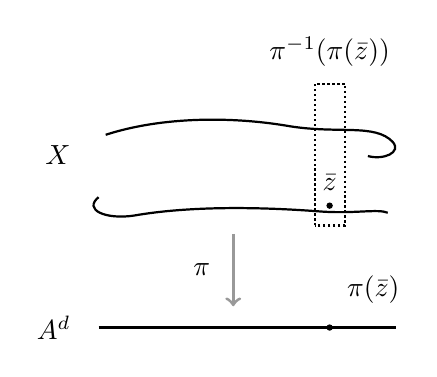
\begin{tikzpicture}[scale=0.9,line width=0.8pt]
  \draw (-1.6,1.30) .. controls (-0.8,1.56) and (0.2,1.56) .. (1.0,1.42)
        .. controls (1.7,1.31) and (2.2,1.46) .. (2.45,1.20)
        .. controls (2.58,1.05) and (2.32,0.94) .. (2.10,1.00);
  \draw (-1.70,0.42) .. controls (-1.92,0.24) and (-1.60,0.10) .. (-1.20,0.16)
        .. controls (-0.40,0.30) and (0.60,0.28) .. (1.40,0.22)
        .. controls (1.90,0.18) and (2.24,0.26) .. (2.38,0.20);
  \draw[densely dotted] (1.35,0.02) rectangle (1.78,2.02);
  \fill (1.56,0.30) circle (0.045);
  \node at (1.56,0.62) {$\bar{\boldsymbol{z}}$};
  \node[anchor=south] at (1.56,2.12) {$\pi^{-1}(\pi(\bar{\boldsymbol{z}}))$};
  \node[anchor=east] at (-1.95,1.02) {$X$};
  \draw[gray!80,line width=1.1pt,->] (0.20,-0.10) -- (0.20,-1.12);
  \node[anchor=east] at (0.02,-0.60) {$\pi$};
  \draw (-1.70,-1.42) -- (2.50,-1.42);
  \fill (1.56,-1.42) circle (0.045);
  \node[anchor=south west] at (1.66,-1.22) {$\pi(\bar{\boldsymbol{z}})$};
  \node[anchor=east] at (-1.95,-1.42) {$\mathbb{A}^d$};
\end{tikzpicture}
\caption{定理~12.2.9 之证明中的关键一步。（依原书手绘图重绘。）}\label{fig:going-down-key-step}
\end{figure}

\textbf{12.2.I.（练习）}\quad 把定理~12.2.9 的证明化归为下述问题。设 $X$ 是一个\trIrreducible{}仿射 $k$-\trVariety，而 $Z$ 是一个\trIrreducible{}的\trClosedSubset，它在所有比 $X$ 小者之中极大（唯一比 $X$ 大的\trIrreducible\trClosedSubset{}就是 $X$ 本身），那么 $\dim Z=\dim X-1$。

为方便起见令 $d=\dim X$。由\trNoetherNormalization~12.2.4，我们有对应于环的一个\trFinite\trExtension{}的有限\trMorphism{} $\pi\colon X\to\mathbb{A}^d$。于是 $\pi(Z)$ 是 $\mathbb{A}^d$ 的一个\trIrreducible\trClosedSubset（有限\trMorphism{}是闭的，\mbox{练习~8.3.L}）。

\textbf{12.2.J.（练习）}\quad 证明：只需证 $\pi(Z)$ 是一张\trHypersurface。（提示：任何\trHypersurface{}的\trDimension{}都是 $d-1$，依据的是关于\trDimension{}与\trTrDeg{}的定理~12.2.1。\mbox{练习~12.1.F}蕴涵 $\dim\pi^{-1}(\pi(Z))=\dim\pi(Z)$。但要当心：一般而言 $Z$ 并不是 $\pi^{-1}(\pi(Z))$。）

现在，若 $\pi(Z)$ 不是\trHypersurface，则它真含于一张\trIrreducible\trHypersurface{} $H$ 之中，于是由\trIntegrallyClosed{}\trIntegralDomain{}的\trFinite\trExtension{}的 Going-Down 定理~12.2.12（我们马上就来证明它），存在 $X$ 的某个真包含 $Z$ 的\trIrreducible\trClosedSubset{} $Z'$，这与 $Z$ 的极大性矛盾。\hfill$\square$

\textbf{12.2.12.\ \trhTheorem{}（\trIntegrallyClosed{}\trIntegralDomain{}的\trFinite\trExtension{}的 Going-Down 定理）。}\ ——\ \emph{设 $\phi\colon B\hookrightarrow A$ 是环的一个\trFinite\trExtension{}（于是 $A$ 是一个有限 $B$-\trModule），$B$ 是\trIntegrallyClosed{}的\trIntegralDomain，而 $A$ 是\trIntegralDomain。那么，给定 $B$ 的嵌套\trPrimeIdeal{} $\mathfrak{q}\subset\mathfrak{q}'$，以及 $A$ 的一个位于 $\mathfrak{q}'$ 之上的\trPrimeIdeal{} $\mathfrak{p}'$（即 $\mathfrak{p}'\cap B=\mathfrak{q}'$），则存在 $A$ 的一个含于 $\mathfrak{p}'$ 之内、位于 $\mathfrak{q}$ 之上的\trPrimeIdeal{} $\mathfrak{p}$。}

照例，你应当为这条陈述勾画一幅几何图景。这条定理通常是在「延长一条理想链」的语境下陈述的，与 Going-Up 定理（\cref{ex:going-up-theorem}）的陈述方式如出一辙，你或许愿意把它想通。（对平坦\trMorphism{}的另一条 Going-Down 定理将在\mbox{练习~24.5.E}中给出。）

把「有限」换成「整」，这条定理在更一般的情形下仍然成立；定理~12.2.12 的这一推广见 [E, p.~291]（「Completion of the proof of 13.9」），或者也可参看 [AtM, Thm.~5.16] 或 [Mat1, Thm.~5(v)]，那里有全然不同的证明。至于 $B$ 的「整闭」假设为何不能省去，[E, Fig.~10.4] 给出了一个例子（以图的形式）。

在证明的过程中，我们将用到下面这条容易的事实。我们现在就可以证明它，但我们把它留到\mbox{练习~12.3.E}，因为它的证明用到源于\mbox{练习~12.3.D}的一个小招。

\textbf{12.2.13.\ \trhProposition{}（\trPrimeIdeal{}回避）。}\ ——\ \emph{设 $\mathfrak{p}_1,\dots,\mathfrak{p}_n$ 是环 $A$ 的\trPrimeIdeal，而 $I$ 是 $A$ 的另一个\trIdeal，不含于任何 $\mathfrak{p}_i$。那么 $I$ 不含于 $\bigcup\mathfrak{p}_i$：存在元素 $f\in I$ 不属于任何 $\mathfrak{p}_i$。}

（你能给这条结果一个几何解读吗？你能想明白它为什么叫「\trPrimeIdeal{}回避」吗？）

\textbf{12.2.14.\ 定理~12.2.12 之证明（\trIntegrallyClosed{}\trIntegralDomain{}的\trFinite\trExtension{}的 Going-Down 定理）。}\quad 证明用的是\trGalois{}理论。令 $L$ 为 $K(A)/K(B)$ 的\textbf{\trNormalClosure}（normal closure），即 $\overline{K(B)}$ 的那个含 $K(A)$、并且在 $\overline{K(B)}/K(B)$ 的任何\trAutomorphism{}下都映到自身的最小子域。令 $C$ 为 $B$ 在 $L$ 中的\trIntegralClosure{}（讨论见\mbox{练习~10.7.I}）。由于 $A\hookrightarrow C$ 是\trIntegralExtension，存在 $C$ 的一个位于 $\mathfrak{q}\subset B$ 之上的\trPrimeIdeal{} $Q$（由 Lying Over 定理~8.2.5），以及 $C$ 的一个含有 $Q$、位于 $\mathfrak{q}'$ 之上的\trPrimeIdeal{} $Q'$（由 Going-Up 定理，\cref{ex:going-up-theorem}）。类似地，存在 $C$ 的一个位于 $\mathfrak{p}'\subset A$ 之上（从而位于 $\mathfrak{q}'\subset B$ 之上）的\trPrimeIdeal{} $P'$。倘若 $P'=Q'$，我们就完工了（只需取 $\mathfrak{p}=Q\cap A$），但情况未必如此。然而，下面的引理~12.2.15 表明：存在 $C$ 在 $B$ 上的一个\trAutomorphism{} $\sigma$，它把 $Q'$ 送到 $P'$；于是 $\sigma(Q)$ 在 $A$ 中的像便派上了用场，证明随之完成。下面这幅图（用几何的语汇画出）或许有帮助。\footnote{译注：图中「?」所标记的，正是那个未知的\trPrimeIdeal{} $\sigma(Q)\cap A$：它落在 $\mathfrak{q}$ 之上，但尚不知道它是否含于 $\mathfrak{p}'$。}
\[
\begin{tikzcd}[row sep=2.8em, column sep=3.2em]
\Spec C/\mathfrak{P}' \ar[drr, hook, bend left=10] \ar[ddd, bend right=24] & & & \\
\Spec C/\mathfrak{Q}' \ar[u, "\sigma"] \ar[r, hook] \ar[d] &
\Spec C/\mathfrak{Q} \ar[r, hook] \ar[dd, bend right=20] &
\Spec C \ar[d] &
L \\
\Spec A/\mathfrak{p}' \ar[r, hook] \ar[d] &
\text{?} \ar[r, hook] \ar[d] &
\Spec A \ar[d] &
K(A) \ar[u, hook] \\
\Spec B/\mathfrak{q}' \ar[r, hook] &
\Spec B/\mathfrak{q} \ar[r, hook] &
\Spec B &
K(B) \ar[u, hook]
\end{tikzcd}
\]

\textbf{12.2.15.\ \trhLemma{}。}\ ——\ \emph{设 $B$ 是\trIntegrallyClosed{}的\trIntegralDomain，$L/K(B)$ 是有限的正规\trFieldExtension，而 $C$ 是 $B$ 在 $L$ 中的\trIntegralClosure。若 $\mathfrak{q}'$ 是 $B$ 的一个\trPrimeIdeal，则 $L/K(B)$ 的自同构传递地作用在 $C$ 的位于 $\mathfrak{q}'$ 之上的诸\trPrimeIdeal{}上。}

这条结果在数论中往往首次亮相，此时取 $B=\mathbb{Z}$，而 $L$ 是 $\mathbb{Q}$ 的一个\trGalois{}扩张。

\emph{证明。}\ 设 $P$ 与 $Q_1$ 是 $C$ 的位于 $\mathfrak{q}'$ 之上的两个\trPrimeIdeal，并令 $Q_2,\dots,Q_n$ 为 $C$ 的与 $Q_1$ \trConjugate{}的诸\trPrimeIdeal{}（即 $Q_1$ 在 $\Aut(L/K(B))$ 下的诸像）。若 $P$ 不是诸 $Q_i$ 中的一员，则 $P$ 不含于任何一个 $Q_i$。（你看出为什么了吗？提示：\mbox{练习~12.1.E} 或\mbox{练习~12.1.F}。）于是由\trPrimeIdeal{}回避（命题~12.2.13），$P$ 不含于它们的并，从而存在某个 $a\in P$ 不含于任何 $Q_i$。这样一来，$a$ 的任何\trConjugate{}都不可能含于 $Q_1$，故范数（norm）$N_{L/K(B)}(a)\in B$ 不含于 $Q_1\cap B=\mathfrak{q}'$。（回想：若 $L/K(B)$ 可分，则范数恰好就是诸\trConjugate{}之积。但即便 $L/K(B)$ 不可分，范数也是诸\trConjugate{}的适当幂次之积，这是因为我们可以把 $L/K(B)$ 分解成一个\trSeparable\trExtension{}再接一个\trPurelyInseparable\trExtension，或者因为我们为该\trExtension{}显式取一组基并算出 $a$ 的范数。关于范数的更多内容见 [Lan, \S VI.5]。）但由于 $a\in P$，它的范数落在 $P$ 中，同时也落在 $B$ 中，从而落在 $P\cap B=\mathfrak{q}'$ 中，得出矛盾。\hfill$\square$

我们以几道练习收尾，供你操练与开窍。

\textbf{12.2.K.（练习／定义）}\quad 设 $X$ 是一个\trFiniteDimensional{}的\trNoetherian{}\trScheme。从 $X$ 的\trUnderlyingSet{}出发定义一个函数 $\dim_X(\cdot)\colon X\to\mathbb{Z}^{\ge0}$：取 $\dim_X p$ 为 $X$ 的含有 $p$ 的那个最大\trIrreducibleComponent{}的\trDimension。我们称之为\textbf{$X$ 在 $p$ 处的\trDimension}（dimension of $X$ at $p$）。（\trhCaveat{}：本定义有别于 [Stacks, tag 0055]。）证明：$\dim_X(\cdot)$ 是\trUpperSemicontinuous{}函数。（回想：从\trTopologicalSpace{} $X$ 到 $\mathbb{R}$ 的函数 $f$ 称为\textbf{\trUpperSemicontinuous}的（upper semicontinuous），若对每个 $x\in\mathbb{R}$，$f^{-1}((-\infty,x))$ 是\trOpenSet。不严格地说：这种函数在取极限时可以向上跳。我们的\trUpperSemicontinuous{}函数将取值于 $\mathbb{Z}$，所以不严格地说，函数会在\trClosedSubset{}上向上跳。类似地，$f$ 称为\textbf{\trLowerSemicontinuous}的（lower semicontinuous），若对每个 $x\in\mathbb{R}$，$f^{-1}((x,\infty))$ 是\trOpenSet。）

\textbf{12.2.16.\ 反复出现的主题：\trSemicontinuity。}\quad \trSemicontinuity{}是代数几何中的一个重要观念。以下是一些例子。
\begin{enumerate}[label=(\roman*)]
  \item 函数之矩阵的\trRank{}（因为\trRank{}会在\trClosedSubset{}上下降，各种判别式在那些地方消失），
  \item \trVariety{}在一点处的\trDimension{}（上文\mbox{练习~12.2.K}），
  \item \trFiber\trDimension{}（定理~12.4.3），
  \item \trFiniteType\trQCSheaf{}的\trRank{}（\mbox{练习~14.3.J}），
  \item 有限\trMorphism{}的\trDegree，视作靶上的函数（\S14.3.4），
  \item \trAlgClosedField{}上的\trVariety{}在\trClosedPoint{}处的\trTangentSpace{}的\trDimension{}（\mbox{练习~21.2.G}），
  \item \trCoherentSheaf{}的\trCohomology{}群的\trRank，在固有平坦\trFamily{}中（\trSemicontinuity{}定理~25.1.1）。
\end{enumerate}
除 (i) 以外全是\trUpperSemicontinuous{}的；(i) 则是\trLowerSemicontinuous{}函数。

\textbf{12.2.L.（练习）}\quad 设 $p$ 是\trLocally\trFiniteType{} $k$-\trScheme{} $X$ 的一个\trClosedPoint。证明：下列三个整数相同：(i) $\dim_X p$（\mbox{练习~12.2.K}）；(ii) $\dim\OO_{X,p}$；(iii) $\operatorname{codim}_Xp$。（我们按显然的方式定义\textbf{\trFiniteType{} $k$-\trScheme{}的\trClosedPoint{}上的\trZariskiTopology}：\trClosedSubset{}由方程切出，如 \S8.4.8。）

\textbf{12.2.M.（练习：\trLocally\trFiniteType{} $k$-\trScheme{}的\trDimension{}被\emph{任何}\trFieldExtension{}保持；见\mbox{练习~12.1.H}(a)）}\quad 设 $X$ 是\trPureDimension{} $n$ 的\trLocally\trFiniteType{} $k$-\trScheme，而 $K/k$ 是一个\trFieldExtension{}（不必\trAlgebraic）。证明：$X_K$ 有\trPureDimension{} $n$。提示：化归到 $X$ 仿射的情形，比如说 $X=\Spec A$。再化归到 $A$ 是\trIntegralDomain{}的情形。证明（用\trAxiomOfChoice）$K/k$ 可以写成一个\trPurelyTranscendental\trExtension（purely transcendental extension）的\trAlgebraic\trFieldExtension。于是由\mbox{练习~12.1.H}(a)，只需处理 $K/k$ \trPurelyTranscendental{}的情形，比如说带\trTranscendenceBase{} $\{e_i\}_{i\in I}$（可以是无限的）。证明 $A_K:=A\otimes_k K$ 是\trIntegralDomain，办法是把它解读为\trIntegralDomain{} $A[\{e_i\}]$ 的某个\trLocalization。若 $t_1,\dots,t_d$ 是 $K(A)/k$ 的一个\trTranscendenceBase，证明 $\{e_i\}\cup\{t_j\}$ 是 $K(A_K)/k$ 的一个\trTranscendenceBase。证明 $\{t_j\}$ 是 $K(A_K)/K$ 的一个\trTranscendenceBase。

\mbox{练习~12.2.M}在概念上很重要。例如，若 $X$ 由一些带 $\mathbb{Q}$ 系数的方程描述，则 $X$ 的\trDimension{}不取决于我们把它当作 $\mathbb{Q}$-\trScheme{}还是 $\mathbb{C}$-\trScheme{}来看待。

\textbf{12.2.17.\ \trhRemark{}。}\quad 与\mbox{练习~12.1.H}不同，\mbox{练习~12.2.M}对 $X$ 有\trFiniteType{}假设。若 $X$ 是任意的\trPureDimension{} $n$ 的 $k$-\trScheme，而 $K/k$ 是任意\trExtension，则 $X_K$ 未必有\trPureDimension{} $n$。例如，\mbox{练习~10.2.L}表明：若 $k$ 是域，则 $\dim k(x)\otimes_k k(y)=1$。

\textbf{12.2.18.}\ \hard\ \textbf{\trHypersurface{}上的直线，第 1 部分。}\quad 注意：虽然维数论并不是下述陈述的中心，它对证明却至关重要。

\textbf{12.2.N.（有启发性的艰苦练习：三维空间中次数 $d>3$ 的\trSurface{}大多没有直线）}\quad 在这道练习中，我们在一个\trAlgClosedField{} $\overline{k}$ 上工作。对任意 $d>3$，证明：$\mathbb{P}^3$ 中大多数次数 $d$ 的\trSurface{}不含直线。这里，「大多数」意指：「四个变量的次数 $d$ \trHomogeneous{}多项式在相差标量倍意义下的参数空间的某个\trZariski\trOpenSet{}的全部\trClosedPoint」。由于这样的\trMonomial{}共有 $\binom{d+3}{3}$ 个，次数 $d$ 的\trHypersurface{}由 $\mathbb{P}^{\binom{d+3}{3}-1}$ 参数化（见注记~4.5.3）。提示：构造一个「\trIncidenceCorrespondence」（incidence correspondence）
\[
X=\{(\ell,H)\ :\ [\ell]\in\mathbb{G}(1,3),\ [H]\in\mathbb{P}^{\binom{d+3}{3}-1},\ \ell\subset H\},
\]
它参数化 $\mathbb{P}^3$ 中含于某张\trHypersurface{}的直线：请定义 $\mathbb{P}^{\binom{d+3}{3}-1}\times\mathbb{G}(1,3)$ 的一个\trClosedSubscheme{} $X$，使这个观念变得精确。（回想 $\mathbb{G}(1,3)$ 是一个\trGrassmannian。）证明：$X$ 是 $\mathbb{G}(1,3)$ 上的一个 $\mathbb{P}^{\binom{d+3}{3}-1-(d+1)}$-丛。（对此的一个可能提示：含直线 $x=y=0$ 的次数 $d$ \trHypersurface{}有多少个？）证明 $\dim\mathbb{G}(1,3)=4$（见 \S7.7：$\mathbb{G}(1,3)$ 有一个由 $\mathbb{A}^4$ 组成的\trOpenCover）。证明 $\dim X=\binom{d+3}{3}-1-(d+1)+4$。证明投射 $X\to\mathbb{P}^{\binom{d+3}{3}-1}$ 的像必含于一个真\trClosedSubset。下面的图或许有帮助。
\[
\dim\bigl(\tbinom{d+3}{3}\bigr)-1-(d+1)+4
\]
\[
\begin{tikzcd}[row sep=3.4em, column sep=5.2em]
& X \ar[dl] \ar[dr, "\mathbb{P}^{\binom{d+3}{3}-1-(d+1)}"] & \\
\mathbb{P}^{\binom{d+3}{3}-1} & & \mathbb{G}(1,3) & \dim 4
\end{tikzcd}
\]
（这一论证很容易推广，用以证明：若 $d>2n-3$，则 $\mathbb{P}^n$ 中「大多数」次数 $d$ 的\trHypersurface{}没有直线。$n=1$ 与 $n=2$ 的情形是平凡的，但值得想上一遍。）

\textbf{12.2.19.\ 旁注。}\quad 倘若你把上一道练习做了，你的维数计数将会提示如下真实的事实：次数 $1$ 的\trHypersurface——即\trHyperplane——具有二维的直线族，而大多数次数 $2$ 的\trHypersurface{}具有一维的直线族（\trRuling），如\mbox{练习~9.3.L}所示。它们还会提示：大多数次数 $3$ 的\trHypersurface{}只含有限多条直线，这正呼应了那个赫赫有名的事实：\trAlgClosedField{}上的正则三次\trSurface{}总含 $27$ 条直线（定理~27.0.1），而我们也将用这个「\trIncidenceCorrespondence」或「\trIncidenceVariety」来证明它（\S27.3）。关于四次\trSurface{}的那个陈述推广为\trNoether{}--\trLefschetz{}定理，它蕴含：一张\textbf{\trVeryGeneral{}的}（very general）、次数 $d\ge4$ 的\trSurface{}不含任何「不是该\trSurface{}与一张\trHypersurface{}之交」的\trCurve；见 [Lef, GH2]。「\trVeryGeneral{}的」意思是：在参数空间（此处即参数化次数 $d$ \trSurface{}的那个\trProjectiveSpace）中，这条陈述在一个可数并的真\trZariski\trClosedSubset{}之外处处成立。与「泛的」（general，定义见 \S10.3.7）一样，「\trVeryGeneral{}的」是「几乎每一个」一语的弱化说法。


\section{克鲁尔定理}

下面我们将引入一批将要反复使用的结果，它们把函数与其消失之处——那些余维数为 $1$ 的点——联系起来。关键的结果是\trKrull{}\trPrincipalIdealTheorem（Principal Ideal Theorem）：它在几何上令人可信，而其证明虽短，却又莫名地不直观而代数化。本节将需要\trNoetherian{}假设。

\textbf{12.3.1.\ \trKrull{}\trPrincipalIdealTheorem。}\quad 在一个\trVectorSpace{}中，单独一个线性方程切出的子空间，其\trCodimension{}总是 $0$ 或 $1$（且\trCodimension{}为 $0$ 仅当方程本身就是 $0$）。\trPrincipalIdealTheorem{}归功于 W.~\trKrull，它推广了这条线性代数事实。

\textbf{12.3.2.\ \trKrull{}\trPrincipalIdealTheorem（几何版本）。}\ ——\ \emph{设 $X$ 是一个\trLocally\trNoetherian\trScheme，$f$ 是一个函数。那么 $V(f)$ 的诸\trIrreducibleComponent{}的\trCodimension{}都是 $0$ 或 $1$。}

这显然是下面这条代数陈述的推论。

\textbf{12.3.3.\ \trKrull{}\trPrincipalIdealTheorem（代数版本）。}\ ——\ \emph{设 $A$ 是一个\trNoetherian{}环，$f\in A$。那么，凡在含 $f$ 的诸\trPrimeIdeal{}之中极小的 $\mathfrak{p}$，其\trCodimension{}至多为 $1$。再者，若 $f$ 不是\trZerodivisor，则每个含 $f$ 的这种 $\mathfrak{p}$，其\trCodimension{}都恰为 $1$。}

例如，\trLocallyPrincipal{}闭子概形具有「余维数 $0$ 或 $1$」，而\trEffectiveCartierDivisor{}具有「纯余维数 $1$」。下面是另一个例子（不用\trPrincipalIdealTheorem{}你当然也能直接证明它）。

\textbf{12.3.A.（练习）}\quad 证明：域 $k$ 上 $n+1$ 个变量的一个\trIrreducible\trHomogeneous{}多项式，描述 $\mathbb{P}^n_k$ 中一个\trDimension{}为 $n-1$ 的\trIntegral\trScheme。

你只须留意\trhTheorem{}~12.3.3 的证明有多短，然后径直跳到 \S12.3.5；等你把这个定理用得足够多、深切体会到它的价值之后，再回头读证明不迟。

\textbf{12.3.4.}\ \extrahard\ \textbf{\trKrull{}\trPrincipalIdealTheorem~12.3.3 之证明。}\quad 我们先料理最后一句：若 $\mathfrak{p}$ 的\trCodimension{}为 $0$，则它是一个\trAssociatedPrimeIdeal（\mbox{练习~6.6.M}），从而它的任何元素（包括 $f$ 在内）都是\trZerodivisor（命题~6.6.13）。

接下来我们要证 $\operatorname{codim}\mathfrak{p}\le1$。我们化归到局部环的情形：把 $A$ 换成 $A_{\mathfrak{p}}$（并把 $\mathfrak{p}$ 换成 $\mathfrak{p}A_{\mathfrak{p}}$）并不改变问题，故可设 $\mathfrak{p}$ 是一个\trMaximalIdeal。

反设 $\mathfrak{q}$ 是 $A$ 的一个严格更小的\trPrimeIdeal（于是由 $\mathfrak{p}$ 在含 $f$ 的诸\trPrimeIdeal{}之中的极小性，$f\notin\mathfrak{q}$）。我们要证 $\mathfrak{q}$ 的\trCodimension{}为 $0$。

证明的关键想法是下面这个巧妙的构造。

\textbf{12.3.B.（练习）}\quad 设 $\phi\colon A\to A_{\mathfrak{q}}$ 是\trLocalization，并定义 $\mathfrak{q}^{(n)}:=\phi^{-1}(\mathfrak{q}^nA_{\mathfrak{q}})$。（它称为 $\mathfrak{q}$ 的第 $n$ 个\textbf{\trSymbolicPower}（symbolic power），但我们不会使用这个术语。）注意 $\mathfrak{q}^{(1)}\supset\mathfrak{q}^{(2)}\supset\cdots$ 是 $A$ 的理想的一个降序列。若 $ag\in\mathfrak{q}^{(n)}$ 而 $g\notin\mathfrak{q}$，证明 $a\in\mathfrak{q}^{(n)}$。（转述：$\mathfrak{q}^{(n)}$ 是 $\mathfrak{q}$-\trPrimary{}的，尽管这个术语我们同样不去用它。）

现在 $\sqrt{(f)}\subset A$ 是含 $f$ 的诸\trMinimalPrimeIdeal{}之交（\cref{ex:radical-intersection-primes}），而这个交恰恰就是\trMaximalIdeal{} $\mathfrak{p}$。于是在局部环 $A/(f)$ 中，\trNilradical{}理想正是\trMaximalIdeal，故由命题~12.1.9（关于\trDimension{}为 $0$ 的\trNoetherian{}局部环），$A/(f)$ 的理想的任何降链都最终恒定。特别地，$\mathfrak{q}^{(1)}\supset\mathfrak{q}^{(2)}\supset\cdots$ 在 $A/(f)$ 中的像最终恒定，于是
\begin{equation*}\tag{12.3.4.1}\label{eq:symbolic-power-congruence}
\mathfrak{q}^{(n)}\equiv\mathfrak{q}^{(n+1)}\pmod{f}\qquad\text{对充分大的 }n\ge n_0.
\end{equation*}
接下来我们断言：事实上对 $n\ge n_0$ 有 $\mathfrak{q}^{(n)}=\mathfrak{q}^{(n+1)}+f\mathfrak{q}^{(n)}$。理由：设 $b_n\in\mathfrak{q}^{(n)}$。那么由式~\eqref{eq:symbolic-power-congruence}，$b_n=b_{n+1}+af$，其中 $b_{n+1}\in\mathfrak{q}^{(n+1)}\subset\mathfrak{q}^{(n)}$，而 $a\in A$。于是 $af\in\mathfrak{q}^{(n)}$；但 $f\notin\mathfrak{q}$。由\mbox{练习~12.3.B}，$a\in\mathfrak{q}^{(n)}$，故正如所断言的，$\mathfrak{q}^{(n)}=\mathfrak{q}^{(n+1)}+f\mathfrak{q}^{(n)}$。

于是，由\trNakayama{}引理~8.2.9（取 $A$，$M=\mathfrak{q}^{(n)}/\mathfrak{q}^{(n+1)}$，$I=(f)$），得 $\mathfrak{q}^{(n)}=\mathfrak{q}^{(n+1)}$，从而 $\mathfrak{q}^nA_{\mathfrak{q}}=\mathfrak{q}^{n+1}A_{\mathfrak{q}}$。再由\trNakayama{}引理~8.2.9（取 $A_{\mathfrak{q}}$，$M=\mathfrak{q}^nA_{\mathfrak{q}}$，$I=\mathfrak{q}A_{\mathfrak{q}}$），得 $\mathfrak{q}^nA_{\mathfrak{q}}=0$，故由命题~12.1.9，$A_{\mathfrak{q}}$ 的\trDimension{}为 $0$，从而 $\mathfrak{q}$ 在 $A$ 中的\trCodimension{}为 $0$，正如所愿。\hfill$\square$

\textbf{12.3.5.}\quad 现在我们用\trKrull{}\trPrincipalIdealTheorem{}来证明几条几何事实。先讲一个有趣的小事实，为\mbox{练习~12.3.D(a)}做准备；它在别的场合也将大有用处。

\textbf{12.3.C.（重要练习，将被反复使用）}\quad 设 $k$ 是一个域（可以是有限的！），$n\in\mathbb{Z}^+$。设 $\{p_1,\dots,p_m\}\subset\mathbb{P}^n_k$\footnote{原书此处作「$\{p_1,\dots,p_m\}\in\mathbb{P}^n_k$」，当系「$\subset$」之误，径改。——译者注}是一族点，不必是闭点。证明：存在一张非空\trHypersurface（次数不作指定），不含任何一个 $p_i$。提示：对 $m$ 作归纳。从 $m$ 到 $m+1$ 的一步：取一张不在 $p_1,\dots,p_m$ 上消失的\trHypersurface。若它在 $p_{m+1}$ 上也不消失，便告完成。否则，记这张\trHypersurface{}为 $f_{m+1}$。再把 $m+1$ 换成每个 $1\le i\le m$ 后如法炮制。然后考虑 $\sum_i f_1\cdots\widehat{f_i}\cdots f_{m+1}$。

\textbf{12.3.D.（重要练习，将被反复使用）}\quad 这是一条很酷的论证。
\begin{enumerate}[label=(\alph*)]
\item \emph{（在射影空间中，\trHypersurface{}与一切\trDimension{}至少为 $1$ 的东西都相交；仿射空间则不然。）}\ 设 $X$ 是 $\mathbb{P}^n_k$ 的一个\trDimension{}至少为 $1$ 的\trClosedSubset，而 $H$ 是 $\mathbb{P}^n_k$ 中一张非空\trHypersurface。证明：$H$ 与 $X$ 相交。（提示：注意 $H$ 上的\trAffine\trCone{}包含 $\mathbb{A}^{n+1}_k$ 的原点。把\trKrull{}\trPrincipalIdealTheorem~12.3.3 应用于 $X$ 上的锥。）
\item 设 $X\hookrightarrow\mathbb{P}^n_k$ 是一个\trDimension{}为 $r$ 的\trClosedSubset。证明：任何\trCodimension{}为 $r$ 的\trLinearSpace{}都与 $X$ 相交。提示：把你在 (a) 中的论证加以精炼。（\mbox{练习~12.3.G}把它推广成：射影空间中凡凭维数理由你预期应当相交的任何两个东西，事实上确实相交。）
\item 再证明：存在一个由 $r+1$ 张非空\trHypersurface{}切出的交，它与 $X$ 不相交。（关键一步：由\mbox{练习~12.3.C}，存在一张次数足够高、不含 $X$ 的任何\trGenericPoint{}的\trHypersurface。）若 $k$ 无限，证明：存在一个\trCodimension{}为 $r+1$ 的\emph{线性子空间}与 $X$ 不相交。（关键一步：证明存在一张\trHyperplane，不含 $X$ 某个分量的任何\trGenericPoint。）
\item 若 $k$ 是无限域，证明：存在一个由 $r$ 张\trHyperplane{}切出的交，它与 $X$ 相交于有限多个点。（我们将在\mbox{练习~13.4.C}中看到：若 $k=\overline{k}$，则对这 $r$ 张\trHyperplane{}的「大多数」选取，这个交是既约的；并在\mbox{练习~18.6.M}中看到：交点个数就是 $X$ 的「次数」。当然，首先我们得定义「次数」。）
\end{enumerate}

\trPrimeIdeal{}回避（即下面这道练习）的证明与\mbox{练习~12.3.D(c)}类似，你或许愿意先把它解出来。我们很快就会发现它有用。

\textbf{12.3.E.（练习）}\quad 证明命题~12.2.13（\trPrimeIdeal{}回避）。提示：对 $n$ 作归纳。别去翻文献——你可能会找到一条长得多的论证。

\textbf{12.3.F.（练习：$\mathbb{A}^n_k$ 中交的余维数之上界）}\quad 设 $k=\overline{k}$ 是一个\trAlgClosedField。设 $X$ 与 $Y$ 是 $\mathbb{A}^d_k$ 中\trCodimension{}分别为 $m$ 与 $n$ 的\trIrreducible{}闭子簇（可以有奇点）。请按如下步骤证明：$X\cap Y$ 的每个分量在 $\mathbb{A}^d_k$ 中的\trCodimension{}至多为 $m+n$。证明：对角子概形 $\mathbb{A}^d_k\cong\Delta\subset\mathbb{A}^d_k\times_k\mathbb{A}^d_k$ 是一个\trCodimension{}为 $d$ 的\trRegularEmbedding。（$\Delta$ 的那 $d$ 个方程你很快就能猜到。）\mbox{练习~11.2.M}把 $X$ 与 $Y$ 在 $\mathbb{A}^d$ 中的交，等同于 $X\times Y$ 与 $\Delta$ 在 $\mathbb{A}^d\times_k\mathbb{A}^d_k$ 中的交。然后证明：局部地，$X\cap Y$ 在 $X\times Y$ 中由 $d$ 个方程切出。使用\trKrull{}\trPrincipalIdealTheorem~12.3.3。你还需要\mbox{练习~12.2.F}。（不可约性假设可以通过适当推广\mbox{练习~12.2.F}而换成纯维性；$k=\overline{k}$ 的假设可以通过适当地动用\mbox{练习~12.1.H}而去掉。推广见\mbox{练习~13.2.N}。）

\textbf{12.3.G.（好玩的练习：推广\mbox{练习~12.3.D(b)}）}\quad 设 $X$ 与 $Y$ 是 $\mathbb{P}^n$ 中\trPureDimensional{}的闭子簇，\trCodimension{}分别为 $d$ 与 $e$，且 $d+e\le n$。证明：$X$ 与 $Y$ 相交。提示：把\mbox{练习~12.3.F}应用于 $X$ 与 $Y$ 的\trAffine\trCone。回想你在\mbox{练习~12.3.D(a)}或 (b) 中用过的论证。

\textbf{12.3.H.（有用的练习）}\quad 设 $f$ 是\trNoetherian{}环 $A$ 的一个元素，不含于任何\trCodimension{}为 $0$ 或 $1$ 的\trPrimeIdeal。证明：$f$ 是\trInvertible{}的。（提示：一个函数若无处消失，它就是\trInvertible{}的，见\cref{ex:vanishing-locus-closed}(b)。）

\textbf{12.3.6.\ \trUFD{}的一个有用的刻画。}\quad 我们可以用\trKrull{}\trPrincipalIdealTheorem，证明 \S5.4.5 中许诺过的\trUFD{}四条有用判别法之一。

\textbf{12.3.7.\ \trhProposition{}。}\ ——\ \emph{设 $A$ 是一个\trNoetherian\trIntegralDomain。那么 $A$ 是\trUFD，当且仅当所有\trCodimension{} $1$ 的\trPrimeIdeal{}都是\trPrincipalIdeal。}

这包含了引理~12.1.7，以及（在某种意义上的）它的逆命题。

\emph{证明。}\ 一个方向就是引理~12.1.7：若 $A$ 是\trUFD，则所有\trCodimension{} $1$ 的\trPrimeIdeal{}都是\trPrincipalIdeal。所以我们反过来假设 $A$ 的所有\trCodimension{} $1$ 的\trPrimeIdeal{}都是\trPrincipalIdeal，并证明 $A$ 是\trUFD。现在，每个\trCodimension{} $1$ 的\trPrimeIdeal{}既然是主理想，便由一个\trPrimeElement{}生成，而这个\trPrimeElement{}在相差一个单位的倍数下是唯一的。\trIntegralDomain{}的所有\trPrimeElement{}都是\trIrreducible{}的，用通常的论证即可。（设 $p\in A$ 是\trPrimeElement，且 $p=ab$，其中 $a,b\in A\setminus\{0\}$。那么由理想 $(p)$ 的素性，$a$ 或 $b$ 落在 $(p)$ 中，比如说无妨设 $a=kp$。于是 $p=kpb$，从而 $1=bk$，从而 $b$ 是单位。故 $p$ 是\trIrreducible{}的。）反之，若 $a\in A$ 是\trIrreducible{}的，则由\trKrull{}\trPrincipalIdealTheorem~12.3.3，$V(a)$ 含有某个\trCodimension{} $1$ 的点 $[(p)]$，于是 $a\in(p)$，比如说 $a=kp$。但由 $a$ 的\trIrreducible{}性，既然 $p$ 不是单位，$k$ 就必是单位，从而 $(a)=(p)$，故 $a$ 是\trPrimeElement。这样我们便证明了：\trPrimeElement{}就是\trIrreducible{}元（并且顺带地，在相差乘法单位的意义下，它们对应于\trCodimension{} $1$ 的\trPrimeIdeal）。最后，由通常的论证（例如 [DF, \S8.3]）：每个非单位的非零元素都可以分解成有限多个\trIrreducible{}元之积，而这种分解的唯一性可以用「这些\trIrreducible{}元同时也是\trPrimeElement」这一事实来证明。\hfill$\square$

\textbf{12.3.8.\ 归纳地使用\trKrull{}\trPrincipalIdealTheorem。}\quad 下面的结果将使我们能够归纳地使用\trKrull{}\trPrincipalIdealTheorem。

\textbf{12.3.9.\ \trhLemma{}。}\ ——\ \emph{设 $\mathfrak{p}_0\subsetneq\mathfrak{p}_1\subsetneq\cdots\subsetneq\mathfrak{p}_n$ 是\trNoetherian{}环 $A$ 中的一条严格\trPrimeIdeal{}链，且 $f\in\mathfrak{p}_n\setminus\mathfrak{p}_0$。那么存在 $A$ 中的一条严格\trPrimeIdeal{}链}
\[
\mathfrak{p}_0=\mathfrak{q}_0\subsetneq\mathfrak{q}_1\subsetneq\cdots\subsetneq\mathfrak{q}_{n-1}\subsetneq\mathfrak{q}_n=\mathfrak{p}_n,
\]
\emph{满足 $f\in\mathfrak{q}_1\setminus\mathfrak{q}_0$。}

你应当立刻感到一股不可抗拒的冲动，要为这条引理勾一幅草图。给定的是 $\Spec A$、一个嵌套的\trIrreducible{}\trClosedSubset{}序列，以及一个包含最小\trClosedSubset{}的「\trHypersurface」。我们要造出一个新的\trIrreducible{}\trClosedSubset{}序列：起点与终点不变，而其中的成员（除第一个之外）全都含于这张\trHypersurface{}之中。

\emph{证明。}\ 我们的计划是按下图来造这些理想：
\[
\begin{tikzcd}[row sep=3.6em, column sep=2.4em]
\mathfrak{p}_0 \ar[r, "\neq"] \ar[rd, "\neq"'] &
\mathfrak{p}_1 \ar[r, "\neq"] \ar[rd, "\neq"'] &
\cdots \ar[r, "\neq"] \ar[rd, "\neq"'] &
\mathfrak{p}_{n-2} \ar[r, "\neq"] \ar[rd, "\neq"'] &
\mathfrak{p}_{n-1} \ar[r, "\neq"] \ar[rd, "\neq"'] &
\mathfrak{p}_n \ar[d, no head, double] \\
f\in & \mathfrak{q}_1 \ar[r, "\neq"'] &
\cdots \ar[r, "\neq"'] &
\mathfrak{q}_{n-2} \ar[r, "\neq"'] &
\mathfrak{q}_{n-1} \ar[r, "\neq"'] &
\mathfrak{q}_n.
\end{tikzcd}
\]

不出所料，我们用递降归纳来做这件事。我们证明如下命题：设 $\mathfrak{p}_{j-2}\subsetneq\mathfrak{p}_{j-1}\subsetneq\mathfrak{p}_j$，且 $f\in\mathfrak{p}_j\setminus\mathfrak{p}_{j-2}$。我们要找的是一个含 $f$ 的\trPrimeIdeal{} $\mathfrak{q}_{j-1}$，满足 $\mathfrak{p}_{j-2}\subsetneq\mathfrak{q}_{j-1}\subsetneq\mathfrak{p}_j$。取 $\mathfrak{q}_{j-1}$ 为一个包含 $(f,\mathfrak{p}_{j-2})$ 的素理想，并且在含于 $\mathfrak{p}_j$ 的那些之中极小。现在，由\trKrull{}\trPrincipalIdealTheorem，$\mathfrak{q}_{j-1}$ 在 $A/\mathfrak{p}_{j-2}$ 中的\trCodimension{}为 $1$，而 $\mathfrak{p}_j$ 的\trCodimension{}至少为 $2$（我们有一条长度为 $2$ 的链 $\mathfrak{p}_{j-2}\subsetneq\mathfrak{p}_{j-1}\subsetneq\mathfrak{p}_j$）。故 $\mathfrak{q}_{j-1}\subsetneq\mathfrak{p}_j$。\hfill$\square$

\textbf{12.3.I.（练习）}\quad 设 $(A,\mathfrak{m})$ 是一个\trNoetherian\trLocalRing，$f\in\mathfrak{m}$。证明：$\dim A/(f)\ge\dim A-1$。

\trKrull{}\trPrincipalIdealTheorem{}的下面这条推广，看上去似乎能由克鲁尔定理归纳地推出，但其实更为微妙。

\textbf{12.3.10.\ \trKrull{}高度定理。}\ ——\ \emph{设 $X=\Spec A$，其中 $A$ \trNoetherian，而 $Z$ 是 $V(f_1,\dots,f_r)$ 的一个\trIrreducibleComponent，这里 $f_1,\dots,f_r\in A$。那么 $Z$ 的\trCodimension{}至多为 $r$。}

（如 \S12.1.4 所述，「\trHeight」是\trCodimension{}的另一个常用说法。）

\textbf{12.3.J.（练习）}\quad 证明\trKrull{}高度定理~12.3.10：先把它化归到\trNoetherian{}局部环 $(A,\mathfrak{m})$ 且 $Z=V(\mathfrak{m})$ 的情形，再对 $f_1,\dots,f_r$ 依次使用引理~12.3.9。

\textbf{12.3.K.（重要练习）}\quad 设 $(A,\mathfrak{m})$ 是一个\trNoetherian\trLocalRing。
\begin{enumerate}[label=(\alph*)]
\item \emph{（\trNoetherian{}局部环的\trDimension{}有限——注记~12.1.11 中所许诺的。）}\ 使用\trKrull{}高度定理~12.3.10 证明：若存在 $g_1,\dots,g_\ell$ 使得 $V(g_1,\dots,g_\ell)=\{[\mathfrak{m}]\}$，则 $\dim A\le\ell$。进而证明：$A$ 具有有限\trDimension。（作为对比，一般的\trNoetherian{}环可以有无限的\trDimension；见\mbox{练习~12.1.M}。）
\item 令 $d=\dim A$。证明：存在 $g_1,\dots,g_d\in A$，使得 $V(g_1,\dots,g_d)=\{[\mathfrak{m}]\}$。
\end{enumerate}

\textbf{12.3.11.}\ \emph{\trhDefinition{}。}\quad 上面这道练习的几何转述如下。给定一点 $p$ 附近的一个 $d$ 维「\trReasonable{}空间的\trGerm」，把 $p$ 集合论地用 $d$ 个方程切出来是办得到的，而且我们总需要至少 $d$ 个方程。$A$ 的这 $d$ 个元素称为 $p$ 处的一个\textbf{\trSystemOfParameters}（system of parameters）。本质上等价地：若 $(A,\mathfrak{m})$ 是一个\trDimension{}为 $d$ 的\trNoetherian\trLocalRing，则 $f_1,\dots,f_d$ 称为 $(A,\mathfrak{m})$ 的一个\textbf{\trSystemOfParameters}，如果 $\mathfrak{m}=\sqrt{(f_1,\dots,f_d)}$。

下面的结果在下一章中将居于中心地位。

\textbf{12.3.12.\ \trhTheorem{}。}\ ——\ \emph{对任何\trNoetherian\trLocalRing{} $(A,\mathfrak{m},k)$，有 $\dim A\le\dim_k\mathfrak{m}/\mathfrak{m}^2$。}

\emph{证明。}\ 现在 $\mathfrak{m}$ 是\trFinitelyGenerated{}的，故 $\mathfrak{m}/\mathfrak{m}^2$ 是一个\trFinitelyGenerated{}的 $(A/\mathfrak{m}=k)$-\trModule，从而是\trFiniteDimensional{}的。设 $\dim_k\mathfrak{m}/\mathfrak{m}^2=n$。取 $\mathfrak{m}/\mathfrak{m}^2$ 的一组基，并把它提升为 $\mathfrak{m}$ 中的元素 $f_1,\dots,f_n$。由\trNakayama{}引理（版本~4，\cref{ex:nakayama-version-4}），$(f_1,\dots,f_n)=\mathfrak{m}$。由\mbox{练习~12.3.K}，$\dim A\le n$。\hfill$\square$

我们以两个带星小节收尾。

\textbf{12.3.13.}\ \hard\ \textbf{「\trCodimension」观念的病理。}\quad 我们可以用\trKrull{}\trPrincipalIdealTheorem，造出本章早先许诺的那桩\trCodimension{}观念的病理例子。令 $A=k[x]_{(x)}[t]$。换句话说，$A$ 的元素是 $t$ 的多项式，其系数是 $x$ 的多项式的商，并且分母中不出现 $x$ 的因子。（\trhWarning{}：$A$ 不是 $k[x,t]_{(x)}$。）显然，$A$ 是一个\trIntegralDomain，故 $xt-1$ 不是\trZerodivisor。你可以验证 $A/(xt-1)\cong k[x]_{(x)}[1/x]\cong k(x)$——「在 $k[x]_{(x)}$ 中，我们本来可以除以除 $x$ 之外的一切，而现在 $x$ 也可以除了」——故 $A/(xt-1)$ 是一个域。于是 $(xt-1)$ 不只是素理想，还是极大理想。由\trKrull{}\trPrincipalIdealTheorem，$(xt-1)$ 的\trCodimension{}为 $1$。从而 $(0)\subset(xt-1)$ 是一条极大的链。然而，$A$ 的\trDimension{}至少为 $2$：$(0)\subset(t)\subset(x,t)$ 是一条长度为 $2$ 的\trPrimeIdeal{}链。（事实上，$A$ 的\trDimension{}恰为 $2$，不过为了观察这桩病理，我们并不需要这个事实。）于是我们有：在一个\trDimension{}为 $2$ 的环里有一个\trCodimension{} $1$ 的素理想，其商的\trDimension{}是 $0$ 而非 $1$。下面是这些理想的偏序集的一幅图。
\[
\begin{tikzpicture}[scale=1.05]
  \node (xt) at (0.2,2.2) {$(x,t)$};
  \node (t) at (-0.15,1.0) {$(t)$};
  \node (xt1) at (2.1,1.0) {$(xt-1)$};
  \node (zer) at (0.9,-0.2) {$(0)$};
  \draw (xt) -- (t);
  \draw (t) -- (zer);
  \draw (xt1) -- (zer);
\end{tikzpicture}
\]

这个例子来自几何，画一幅图是富有启发性的；见\cref{fig:codim-pathology}。$\Spec k[x]_{(x)}$ 对应于 $\mathbb{A}^1_k$ 在原点附近的一个「\trGerm」，而 $\Spec k[x]_{(x)}[t]$ 则对应于「它 $\times$ \trAffineLine」。你也许能从图中看出这桩病理的某种缘由——$V(xt-1)$ 与 $V(x)$ 不相交，所以它不能在 $V(x)$ 上有任何\trSpecialization，而 $V(xt-1)$ 也无处可供\trSpecialization{}了。这种不良行为竟然出现在一个看上去相当良性的环里，实在令人不安。

\begin{figure}[htbp]
\centering
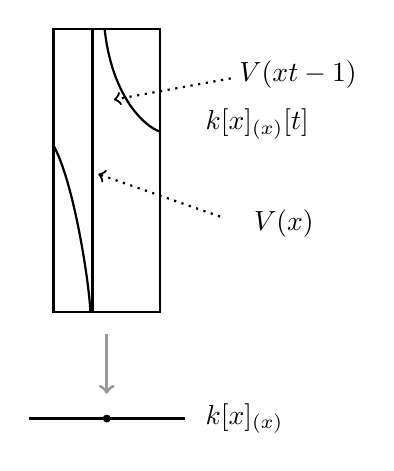
\begin{tikzpicture}[scale=0.9,line width=0.8pt]
  \draw (0,0) rectangle (1.5,4);
  \draw (0.55,0) -- (0.55,4);
  \draw (0.72,4) .. controls (0.82,3.05) and (1.28,2.62) .. (1.5,2.55);
  \draw (0,2.35) .. controls (0.28,1.85) and (0.5,0.45) .. (0.52,0);
  \node at (3.45,3.35) {$V(xt-1)$};
  \draw[dotted,->] (2.5,3.3) -- (0.85,3.0);
  \node at (3.25,1.25) {$V(x)$};
  \draw[dotted,->] (2.35,1.35) -- (0.63,1.95);
  \node[anchor=west] at (2.0,2.65) {$\Spec k[x]_{(x)}[t]$};
  \draw[gray!80,line width=1.1pt,->] (0.75,-0.3) -- (0.75,-1.15);
  \draw (-0.35,-1.5) -- (1.85,-1.5);
  \fill (0.75,-1.5) circle (1.6pt);
  \node[anchor=west] at (2.0,-1.5) {$\Spec k[x]_{(x)}$};
\end{tikzpicture}
\caption{\trSurface{} $\Spec k[x]_{(x)}[t]$ 上\trDimension{}与\trCodimension{}表现得古怪。（依原书手绘图重绘。）}\label{fig:codim-pathology}
\end{figure}

\textbf{12.3.14.}\ \hard\ \textbf{\trHypersurface{}上的直线，第 2 部分。}\quad （第 1 部分为 \S12.2.18。）现在我们给出\trKrull{}\trPrincipalIdealTheorem~12.3.3 的一个几何应用，借\mbox{练习~12.3.D(a)}加以施展。本小节全程在代数闭域 $\overline{k}$ 上工作。

\textbf{12.3.L.（练习）}
\begin{enumerate}[label=(\alph*)]
\item 设
\[
f(x_0,\dots,x_n)=f_d(x_1,\dots,x_n)+x_0f_{d-1}(x_1,\dots,x_n)+\cdots+x_0^{d-1}f_1(x_1,\dots,x_n)
\]
是一个齐次的 $d$ 次多项式（于是 $\deg f_i=i$），它在 $\mathbb{P}^n$ 中切出一张含 $p:=[1,0,\dots,0]$ 的\trHypersurface{} $X$。证明：存在过 $p$ 且含于 $X$ 的直线，当且仅当 $f_1=f_2=\cdots=f_d=0$ 在 $\mathbb{P}^{n-1}=\Proj\overline{k}[x_1,\dots,x_n]$ 中有公共零点。（提示：给定一个公共零点 $[a_1,\dots,a_n]\in\mathbb{P}^{n-1}$，证明连接 $p$ 与 $[0,a_1,\dots,a_n]$ 的直线含于 $X$。）
\item 若 $d\le n-1$，证明：过 $X$ 的任何一点 $p$，都有含于 $X$ 的直线。提示：\mbox{练习~12.3.D(a)}。
\item 若 $d\ge n$，证明：对 $\mathbb{P}^n$ 中「大多数」次数 $d$ 的\trHypersurface{} $X$（意即：凡其对应的点在参数空间 $\mathbb{P}^{\binom{n+d}{d}-1}$ 中落在某个非空\trZariski\trOpenSet{}内的\trHypersurface——参看注记~4.5.3 与\mbox{练习~9.3.J}——都算），「大多数点 $p\in X$」（即 $X$ 的某个非空稠密\trZariski\trOpenSet{}中的全部点）都没有 $X$ 中的直线经过。（提示：先证明存在单独某个 $X$ 中单独一点 $p$，没有任何直线经过它。\trChevalley{}定理~8.4.2 或许可派上用场。）
\end{enumerate}

\textbf{12.3.15.}\ \emph{\trhRemark{}。}\quad 射影（或\trProper）的 $k$-\trVariety{} $X$ 称为\textbf{\trUniruled}的（uniruled），若每一点 $p\in X$ 都含于某个 $\mathbb{P}^1\subset X$。（这个词出了本注记我们就不用了。）(b) 表明：所有次数至多为 $n-1$ 的\trHypersurface{}都是\trUniruled{}的。我们还能证明（要用到超出我们现有所知的方法；见 [Ko1, Cor.~IV.1.11]）：若 $\operatorname{char}\overline{k}=0$，则 $\mathbb{P}^n_k$ 中每张次数至少为 $n+1$ 的\trSmooth\trHypersurface{}都\emph{不}是\trUniruled{}的（这就把 (c) 中的那个开集显式化了）。此外，次数恰为 $n$ 的\trSmooth\trHypersurface{}\emph{确}是\trUniruled{}的，只是覆盖它的是二次曲线而非直线。于是，\trHypersurface{}的行为随着其次数相对 $n+1$ 的位置而有强烈的不同；这一点在许多别的方面也同样成立。次数小于 $n+1$ 的\trSmooth\trHypersurface{}是 \emph{Fano} \trVariety{}的例子；次数为 $n+1$ 的\trSmooth\trHypersurface{}是 \emph{Calabi--Yau} \trVariety{}的例子（依定义之不同，$n=1$ 的情形可能例外）；而次数大于 $n+1$ 的\trSmooth\trHypersurface{}则是\emph{一般型}（general type）\trVariety{}的例子。这些术语我们将在 \S21.5.5 中定义。


\section{簇的态射纤维的维数}

在本节中，我们将证明：\trVariety{}的\trMorphism{}之\trFiber{}的\trDimension，其表现方式正如你从几何直觉所期待的那样。我们直到此刻才来讨论它的原因是：我们将用到定理~12.2.9（对\trVariety{}而言，\trCodimension{}是\trDimension{}之差）。

在动手之前，先确保我们与直觉处在同一页上。消元理论（定理~8.4.10）告诉我们：投射 $\pi\colon\mathbb{P}^{\mathfrak{n}}_A\to\Spec A$ 是闭的。我们可以这样解读这件事：$\mathbb{P}^{\mathfrak{n}}_A$ 的一个\trClosedSubset{} $X$ 由 $\mathfrak{n}+1$ 个变量的一组齐次方程（在 $A$ 上）切出。$X$ 的\trImage{}就是 $\Spec A$ 中这些方程具有公共非平凡解的那个子集。只要肯下功夫，我们就可以把这件事说成：非平凡解的\emph{存在性}（或者在 $\pi\colon X\to\Spec A$ 之下某点存在原像这件事）是一桩「\trUpperSemicontinuous」的事实。更一般地，你的直觉或许会告诉你：$A$ 上 $\mathfrak{n}+1$ 个变量的一组齐次多项式，其解空间（在 $\mathbb{P}^{\mathfrak{n}}_A$ 中）\trDimension{}至少为 $\mathrm{d}$ 的那个\trLocus，应当是 $\Spec A$ 的一个\trClosedSubset。（作为一个特例，考虑线性方程：$\mathfrak{n}+1$ 个变量的 $\mathfrak{m}$ 个线性方程具有\trDimension{}至少为 $\mathrm{d}+1$ 的解空间，这一条件是系数上的一个闭条件——你能借助线性代数看出为什么吗？）这个直觉将是正确的，而且将以一种根本的方式用到\trProperness（定理~12.4.3(b)）。我们还将阐明\emph{源}上\trFiber\trDimension{}的\trUpperSemicontinuous{}性（定理~12.4.3(a)）。一个值得想透的有用例子是从 $xy$-平面到 $xz$-平面的\trMap（$\Spec k[x,y]\to\Spec k[x,z]$），由 $(x,z)\mapsto(x,xy)$ 给出。（这个例子也曾在 \S8.4.1 中出现过。）

我们实质性的讨论，从一条在\trLocally\trNoetherian{}设定下更一般地成立的不等式开始。

\textbf{12.4.A.（关键练习：\trCodimension{}对\trMorphism{}的表现正如你所期待，或「\trFiber\trDimension{}绝不会低于预期」）}\quad 设 $\pi\colon X\to Y$ 是\trLocally\trNoetherian{}\trScheme{}之间的一个\trMorphism，而 $\mathfrak{p}\in X$ 与 $\mathfrak{q}\in Y$ 是满足 $\mathfrak{q}=\pi(\mathfrak{p})$ 的两点。证明：
\[
\operatorname{codim}_X\mathfrak{p}\le\operatorname{codim}_Y\mathfrak{q}+\operatorname{codim}_{\pi^{-1}(\mathfrak{q})}\mathfrak{p}
\]
（见\cref{fig:codim-fiber-inequality}）。（这与\mbox{练习~12.1.K}相似，但它并不相同！）提示：取 $\mathfrak{q}$「在 $Y$ 中」的一组\trSystemOfParameters（定义~12.3.11），再取 $\mathfrak{p}$「在 $\pi^{-1}(\mathfrak{q})$ 中」的一组\trSystemOfParameters，并用它们找出 $\OO_{X,\mathfrak{p}}$ 的 $\operatorname{codim}_Y\mathfrak{q}+\operatorname{codim}_{\pi^{-1}(\mathfrak{q})}\mathfrak{p}$ 个元素，使它们在 $\Spec\OO_{X,\mathfrak{p}}$ 中切出 $\mathfrak{p}=[\mathfrak{m}]$。用\mbox{练习~12.3.K}。

\begin{figure}[htbp]
\centering
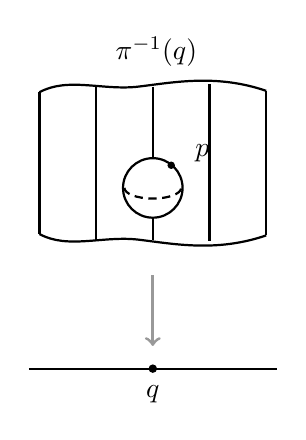
\begin{tikzpicture}[scale=0.9,line width=0.8pt]
  \draw (-1.6,1.0) .. controls (-1.2,1.22) and (-0.7,1.02) .. (-0.2,1.08)
        .. controls (0.3,1.14) and (0.9,1.26) .. (1.6,1.02);
  \draw (-1.6,-1.0) .. controls (-1.2,-1.22) and (-0.7,-1.02) .. (-0.2,-1.08)
        .. controls (0.3,-1.14) and (0.9,-1.26) .. (1.6,-1.02);
  \draw (-1.6,1.0) -- (-1.6,-1.0);
  \draw (1.6,1.02) -- (1.6,-1.02);
  \draw (-0.8,1.10) -- (-0.8,-1.08);
  \draw (0.8,1.12) -- (0.8,-1.10);
  \draw (0,1.08) -- (0,-1.08);
  \filldraw[fill=white] (0,-0.35) circle (0.42);
  \draw[densely dashed] (-0.40,-0.35) arc[start angle=180, end angle=360, x radius=0.40, y radius=0.15];
  \fill (0.26,-0.03) circle (1.5pt);
  \node at (0.70,0.14) {$\mathfrak{p}$};
  \node[anchor=south] at (0.05,1.22) {$\pi^{-1}(\mathfrak{q})$};
  \draw[gray!80,line width=1.1pt,->] (0,-1.58) -- (0,-2.58);
  \draw (-1.75,-2.90) -- (1.75,-2.90);
  \fill (0,-2.90) circle (1.7pt);
  \node at (0,-3.26) {$\mathfrak{q}$};
\end{tikzpicture}
\caption{\mbox{练习~12.4.A}：全空间中一点的\trCodimension，被「该点在\trFiber{}中的\trCodimension」与「其\trImage{}在靶中的\trCodimension」之和所界。（依原书手绘图重绘。）}\label{fig:codim-fiber-inequality}
\end{figure}

\mbox{练习~12.4.A}与你的几何直觉相合吗？你应当能举出一些富有启发性的例子：既有等号成立的，也有等号失败的。我们将看到：对足够好的——即\trFlat{}的——\trMorphism，等号总成立；见命题~24.5.6。

现在我们来证明：\mbox{练习~12.4.A}的不等式在「$Y$ 的大部分」之上其实取等号。

\textbf{12.4.1.\ \trhTheorem。}\ ——\ \emph{设 $\pi\colon X\to Y$ 是\trIntegral{}\trScheme{}之间的一个\trFiniteType{}\trDominant{}\trMorphism，使得有限生成的\trFieldExtension{} $K(X)/K(Y)$ 具有\trTrDeg{} $\mathfrak{r}$。那么存在一个非空\trOpenSubset{} $\mathsf{U}\subset Y$，使得对一切 $\mathfrak{q}\in\mathsf{U}$，$\mathfrak{q}$ 之上的\trFiber{}非空，且具有\trPureDimension{} $\mathfrak{r}$。}

一个有趣的事实：我们将在证明中使用\trNoetherNormalization{}引理~12.2.4，尽管这条陈述并不涉及\trVariety！如果这条陈述的如此一般性让你介意，我们为\trVariety{}准备了下面的特例。

\textbf{12.4.2.\ \trhCorollary。}\ ——\ \emph{设 $\pi\colon X\to Y$ 是不可约 $k$-\trVariety{}之间的一个（必然\trFiniteType{}的）\trMorphism，$\dim X=\mathfrak{m}$ 而 $\dim Y=\mathfrak{n}$。那么存在一个非空\trOpenSubset{} $\mathsf{U}\subset Y$，使得对一切 $\mathfrak{q}\in\mathsf{U}$，$\mathfrak{q}$ 之上的\trFiber{}具有\trPureDimension{} $\mathfrak{m}-\mathfrak{n}$，或者为空。}

（按约定，空集严格按字面也具有\trPureDimension{} $\mathfrak{r}$——空集的每个\trIrreducibleComponent{}都具有\trDimension{} $\mathfrak{r}$。这使推论~12.4.2 的陈述干净了一点。）

\textbf{12.4.B.（练习）}\quad 验证：定理~12.4.1 蕴涵推论~12.4.2。

\emph{\trhTheorem{}~12.4.1 之证明。}\quad 我们从两个快速的化归开始。(i) 必要时缩小 $Y$，便可设 $Y$ 仿射，比如说 $\Spec B$。(ii) 同样还可设 $X$ 仿射，比如说 $\Spec A$。（理由：以有限多个\trAffine\trOpenSubset{} $X_1,\dots,X_a$ \trCover{} $X$，再对每个 $\pi|_{X_i}$ 取相应诸 $\mathsf{U}$ 的交。）

为了给论证的其余部分提供动机，我们先来描述目标。我们将造出 $\Spec B$ 的一个非空\trDistinguishedOpen{} $\mathsf{U}$，使得 $\pi^{-1}(\mathsf{U})\to\mathsf{U}$ 穿过 $\mathbb{A}^{\mathfrak{r}}_{\mathsf{U}}$ 分解，且所经的是一个有限满\trMorphism：
\begin{equation*}\tag{12.4.2.1}\label{eq:finite-surjective-factorization}
\begin{tikzcd}[row sep=2.6em, column sep=4.4em]
X=\Spec A & \pi^{-1}(\mathsf{U}) \ar[l, hook, "\text{开嵌入}"'] \ar[d, "\text{有限满}"] \\
 & \mathbb{A}^{\mathfrak{r}}_{\mathsf{U}} \ar[d] \\
Y=\Spec B \ar[uu, "\pi"] & \mathsf{U}. \ar[l, hook, "\text{开嵌入}"']
\end{tikzcd}
\end{equation*}

\textbf{12.4.C.（练习）}\quad 证明：这就足以证明定理~12.4.1。提示：设 $\mathfrak{p}\in\mathsf{U}$ 是一点，其\trResidueField{}为 $\kappa$。证明：任何有限地映到 $\mathbb{A}^{\mathfrak{r}}_{\kappa}$ 的不可约\trVariety{}都有至多为 $\mathfrak{r}$ 的\trDimension。这将表明 $\pi^{-1}(\mathfrak{p})$ 的任何分量的\trDimension{}至多为 $\mathfrak{r}$。为了证明等号，对 $\Spec A\to\Spec B[x_1,\dots,x_{\mathfrak{r}}]$ 恰当地应用 Going-Down 定理~12.2.12。

于是，我们现在就来着手搭建交换图~\eqref{eq:finite-surjective-factorization}。我们首先注意到：$B$ 含入 $A$ 与 $K(B)$ 二者，而 $A$ 与 $K(B)$ 又都含入 $K(A)$。从 $A$ 与 $K(B)$ 到 $K(A)$ 的这两个映射都穿过 $A\otimes_B K(B)$ 分解（它的 $\Spec$ 就是 $\pi$ 的\trGenericFiber），故从 $A$ 与 $K(B)$ 到 $A\otimes_B K(B)$ 的映射必为包含。
\begin{equation*}\tag{12.4.2.2}\label{eq:generic-fiber-inclusions}
\begin{tikzcd}[row sep=2.6em, column sep=3.8em]
 & & K(A) \\
A \ar[urr, bend left=8] \ar[rr, hook, "\therefore\hookrightarrow"'] & & A\otimes_B K(B) \ar[u] \\
B \ar[u, hook] \ar[rr, hook] & & K(B) \ar[u, hook, "\therefore\hookrightarrow"] \ar[uu, bend right=32]
\end{tikzcd}
\end{equation*}

显然，$K(A)\otimes_B K(B)=K(A)$（因为 $A\otimes_B K(B)$ 可以解读为：取 $A$，并把其中身为 $B$ 的非零元的那些元素全部可逆化），而 $A\otimes_B K(B)$ 是域 $K(B)$ 上\trFinitelyGenerated{}的一个\trAlgebra。

由\trNoetherNormalization~12.2.4，我们可以找到元素 $t_1,\dots,t_{\mathfrak{r}}\in A\otimes_B K(B)$，它们在 $K(B)$ 上\trAlgebraicallyIndependent，使得 $A\otimes_B K(B)$ 在 $K(B)[t_1,\dots,t_{\mathfrak{r}}]$ 上整。

现在，我们可以把诸元素 $t_i\in A\otimes_B K(B)$ 想成分数：分子在 $A$ 中，分母在 $B$ 中（并且非零）。设 $f$ 是各个 $t_i$ 所出现的那些分母之积，那么把 $B$ 换成 $B_f$（即把 $\Spec B$ 换成它的\trDistinguishedOpen{} $D(f)$）之后，便可设诸 $t_i$ 全都落在 $A$ 中。于是（在草率地把 $B_f$ 重命名为 $B$、把 $A_f$ 重命名为 $A$ 之后），我们可以把交换图~\eqref{eq:generic-fiber-inclusions} 修剪并扩充成下面的样子。
\[
\begin{tikzcd}[row sep=2.6em, column sep=4.2em]
A \ar[r, hook] & A\otimes_B K(B) \\
B[t_1,\dots,t_{\mathfrak{r}}] \ar[u, hook] \ar[r, hook] & K(B)[t_1,\dots,t_{\mathfrak{r}}] \ar[u, hook, "\text{整}"'] \\
B \ar[u, hook] \ar[r, hook] & K(B)
\end{tikzcd}
\]

现在 $A$ 在 $B$ 上\trFinitelyGenerated，从而在 $B[t_1,\dots,t_{\mathfrak{r}}]$ 上也\trFinitelyGenerated。然而我们还不能确信 $A$ 在 $B[t_1,\dots,t_{\mathfrak{r}}]$ 上\emph{\trFinite}，所以事情尚未了结。我们将不得不进一步对 $B$ 取\trLocalization。

设 $A$ 在 $B$ 上由 $u_1,\dots,u_{\mathfrak{q}}$ 生成\footnote{原书以记号 $\mathfrak{q}$ 计生成元个数（又如 $F_{\mathfrak{n}}$、$\mathbb{P}^{\mathfrak{n}}_A$ 以维数 $\mathfrak{n}$ 计仿射片数），与全书惯用斜体下标之例不合，兹照录原书。——译者注}。我们的\trNoetherNormalization{}论证蕴涵：每个 $u_i$ 都满足某个首一方程 $f_i(u_i)=0$，其中 $f_i\in K(B)[t_1,\dots,t_{\mathfrak{r}}][t]$（即：把 $f_i$ 视作 $t$ 的、系数取自 $K(B)[t_1,\dots,t_{\mathfrak{r}}]$ 的多项式时，它是首一的）。诸 $f_i$ 的系数（视作 $t_1,\dots,t_{\mathfrak{r}}$ 与 $t$ 的多项式时）先验地是 $B$ 中的分式，但只要乘上全部那些分母，便可设每个 $f_i\in B[t_1,\dots,t_{\mathfrak{r}}][t]$，代价是丧失诸 $f_i$ 的首一性（这一次是视作 $t$ 的多项式而言）。令 $b\in B$ 为诸 $f_i$ 的首项系数（视作 $t$ 的多项式时）之积。若 $\mathsf{U}=D(b)$（即 $b$ 可逆的那个\trLocus），则在 $\mathsf{U}$ 之上，诸 $f_i$（可以取成）具有首项系数 $1$，于是诸 $u_i$（作为 $A_b$ 中的元素）在 $B_b[t_1,\dots,t_{\mathfrak{r}}]$ 上整。从而 $\Spec A_b\to\Spec B_b[t_1,\dots,t_r]$ 既\trFinite{}又满（后者由 Lying Over 定理~8.2.5）。

至此，我们已如所需造出交换图~\eqref{eq:finite-surjective-factorization}。\hfill$\square$

关于这个证明，有几点值得指出。首先，这条结果最初的动机虽然来自域 $k$ 上的经典\trVariety，证明却用到了\emph{另一个}域——\trFunctionField{} $K(B)$——之上的\trVariety{}论。这正是一个例证，说明把\trGenericPoint{}引进\trAlgebraicGeometry{}大有用处，即便在考虑更「经典」的问题时也是如此。

其次，论证主体部分的想法是：我们在\trGenericPoint{}处有一条结果（$\Spec A\otimes_B K(B)$ 在 $K(B)$ 上的仿射空间之上既\trFinite{}又满），而我们想把它「铺展」到 $\Spec B$ 的\trGenericPoint{}的一个\trOpen\trNeighborhood{}上去。我们的做法是：注意到只要把问题正确地描述出来，就会出现「有限多个分母」，然后把这些分母可逆化。这种「铺展」的想法是一个反复出现的主题。

\textbf{12.4.D.（练习：不可约性的有用判别法）}\quad 设 $\pi\colon X\to Y$ 是到一个不可约\trVariety{}上的一个\trProper{}\trMorphism，而 $\pi$ 的全部\trFiber{}都非空，且都不可约并具有相同的\trDimension。证明：$X$ 不可约。

\textbf{12.4.3.\ \trhTheorem{}（\trFiber\trDimension{}的\trUpperSemicontinuous{}性）。}\ ——\ \emph{设 $\pi\colon X\to Y$ 是\trFiniteType{} $k$-\trScheme{}之间的一个\trMorphism。}
\begin{enumerate}[label=(\alph*)]
\item （\emph{源上的\trUpperSemicontinuous{}性}）$\pi$ 在 $\mathfrak{p}\in X$ 处的\trFiber{}的\trDimension{}（即 $\pi^{-1}(\pi(\mathfrak{p}))$ 中含有 $\mathfrak{p}$ 的那个最大分量的\trDimension）作为 $\mathfrak{p}$ 的函数（也就是说，在 $X$ 上）是\trUpperSemicontinuous{}的。
\item （\emph{靶上的\trUpperSemicontinuous{}性}）再者，若 $\pi$ 还是闭的（例如 $\pi$ \trProper），则 $\pi$ 在 $\mathfrak{q}\in Y$ 之上的\trFiber{}的\trDimension{}作为 $\mathfrak{q}$ 的函数（也就是说，在 $Y$ 上）是\trUpperSemicontinuous{}的。
\end{enumerate}
若把闭性假设去掉，你应当能够立刻为 (b) 构造出一个反例。（我们还提一句：对射影\trMorphism{}而言，定理~12.4.3(b) 已在\mbox{练习~18.1.B}中以简单的方式完成了。）

\emph{证明。}\ (a) 令 $F_{\mathfrak{n}}$ 为 $X$ 的由\trFiber\trDimension{}至少为 $\mathfrak{n}$ 的点组成的子集。我们希望证明：对一切 $\mathfrak{n}$，$F_{\mathfrak{n}}$ 都是\trClosedSubset。我们对 $\dim Y$ 作归纳。基底情形 $\dim Y=0$ 是平凡的。于是固定 $Y$，并假设结果对所有维数更小的靶已知。

\textbf{12.4.E.（练习）}\quad 证明：只需在 $X$ 与 $Y$ 都\trIntegral、且 $\pi$ \trDominant{}的情形下证明这条结果。

令 $\mathfrak{r}=\dim X-\dim Y$ 为 $\pi$ 的「相对维数」。若 $\mathfrak{n}\le\mathfrak{r}$，则由\mbox{练习~12.4.A}（再结合定理~12.2.9，即对\trVariety{}而言\trCodimension{}是\trDimension{}之差），有 $F_{\mathfrak{n}}=X$。

若 $\mathfrak{n}>\mathfrak{r}$，则令 $\mathsf{U}\subset Y$ 为定理~12.4.1 中那个「\trFiber\trDimension{}恰为 $\mathfrak{r}$」的\trDense\trOpenSubset。那么 $F_{\mathfrak{n}}$ 与 $\mathsf{U}$ 的原像不相交。把 $Y$ 换成 $Y\setminus\mathsf{U}$（并把 $X$ 换成 $X\setminus\pi^{-1}(\mathsf{U})$）之后，由归纳假设便告完成。

\textbf{12.4.F.（容易的练习）}\quad 证明 (b)（利用 (a)）。\hfill$\square$

\textbf{12.4.4.\ \trhProposition{}（「\trGenericallyFinite{}蕴涵泛有限」；参看\mbox{练习~10.3.G}）。}\ ——\ \emph{设 $\pi\colon X\to Y$ 是\trDimension{}为 $\mathfrak{n}$ 的不可约 $k$-\trVariety{}之间的一个\trGenericallyFinite{}\trMorphism。那么存在一个\trDense\trOpenSubset{} $\mathsf{V}\subset Y$，使 $\pi$ 在其上\trFinite。}

（如果你愿意，日后可以把不可约性假设放宽为只要求 $X$ 与 $Y$ 具有\trPureDimension{} $\mathfrak{n}$。）

\emph{证明。}\ 如同定理~12.4.1 的证明，我们可以设 $Y$ 仿射，且 $\pi$ \trDominant。设 $X=\bigcup_{i=1}^{\mathfrak{n}}\mathsf{U}_i$\footnote{原书此处上标用维数记号 $\mathfrak{n}$ 计仿射片个数，兹照录原书。——译者注}，其中诸 $\mathsf{U}_i$ 是 $X$ 的\trAffine\trOpenSubscheme。由\mbox{练习~10.3.G}，存在\trDense\trOpenSubset{} $\mathsf{V}_i\subset Y$，使得 $\pi|_{\mathsf{U}_i}$ 在其上\trFinite。把 $Y$ 换成 $\bigcap_i\mathsf{V}_i$ 的一个仿射开子集之后，便可设诸 $\pi|_{\mathsf{U}_i}$ 都\trFinite。

\textbf{12.4.G.（练习）}\quad 证明：$\pi$ 是闭的。提示：你只需要用到 $\pi|_{\mathsf{U}_i}$ 是闭的，以及 $\mathsf{U}_i$ 只有有限多个。

于是 $X\setminus\mathsf{U}_1$ 是一个\trClosedSubset，从而 $\pi(X\setminus\mathsf{U}_1)$ 是闭的。

\textbf{12.4.H.（练习）}\quad 证明：这个闭子集并非整个 $Y$。

令 $\mathsf{V}:=Y\setminus\pi(X\setminus\mathsf{U}_1)$。那么 $\pi$ 在 $\mathsf{V}$ 之上\trFinite：它是把有限\trMorphism{} $\pi|_{\mathsf{U}_1}\colon\mathsf{U}_1\to Y$ 限制到靶 $Y$ 的\trOpenSubset{} $\mathsf{V}$ 上所得的\trMorphism。\hfill$\square$

